\documentclass[article,colorback,accentcolor=tud3c]{report}
\usepackage[sumlimits] {amsmath}
\usepackage[utf8]{inputenc}
\usepackage[T1]{fontenc}
\usepackage[ngerman]{babel}
\usepackage[stable]{footmisc}
\usepackage[ngerman]{hyperref}
\usepackage{longtable}
\usepackage{multirow}
\usepackage{booktabs}
\usepackage{graphicx}
\usepackage{caption}
\usepackage{float}
\usepackage{units}
\usepackage{upgreek}
\usepackage{mathtools}
\usepackage{subfigure}
\usepackage{pdfpages}
\usepackage[abs]{overpic}
\usepackage{pict2e}
\usepackage[fixlanguage]{babelbib}
\usepackage{fancyhdr}
\usepackage{layout}


\usepackage{ltxcmds}
\makeatletter
\newcommand*{\getdata}[2]{%
  \expandafter\ltx@CarNumth\expandafter{%
    \the\numexpr(#1)\expandafter
  }#2\@nil
}
\makeatother

\newcommand*{\ktaneChapterNames}{{F}{W}{4}{>6}{T}{S}{B}{E}{O}{N}{A}}



% make @ a letter so we can use it in names of command sequences:
\makeatletter
% call the internal \c@<counter> command and apply number formatting:
\newcommand*\ktaneChapter[1]{\expandafter\@ktaneChapter\csname c@#1\endcsname}
% number formatting:
\newcommand*\@ktaneChapter[1]{\getdata{\the\numexpr(#1)}\ktaneChapterNames\relax}

% make @ other again:
\makeatother

\renewcommand\thesection{\ktaneChapter{section}}
\renewcommand\thesubsection{\thesection.\arabic{subsection}}

\renewcommand\headrule{}

\newcommand\invisiblesection[1]{%
  \cleardoublepage
  \refstepcounter{section}%
  \addcontentsline{toc}{section}{\protect\numberline{\thesection}#1}%
  \sectionmark{#1}}

\pagestyle{fancy}
\fancyhf{}

\setlength{\footskip}{10pt}
\setlength{\textheight}{630pt}


\lfoot{\fancyplain{}{\rightmark}}
\rfoot{\fancyplain{}{\thepage}}


\begin{document}


%Preface
 \includepdf[pages=1-3]{pdf/sections.pdf}

\tableofcontents

\invisiblesection{Few Modules}
 \includepdf[scale=0.9,pages=4,pagecommand={}]{pdf/sections.pdf}

\newpage
\thispagestyle{empty}
\mbox{}

\newpage
\vspace*{-4cm}
\centerline{
\begin{overpic}[scale=1.0,unit=1mm,page=6]{pdf/vanilla.pdf}
    \put(160,20){
\includegraphics{attention.png}}
\end{overpic}
}

\newpage
 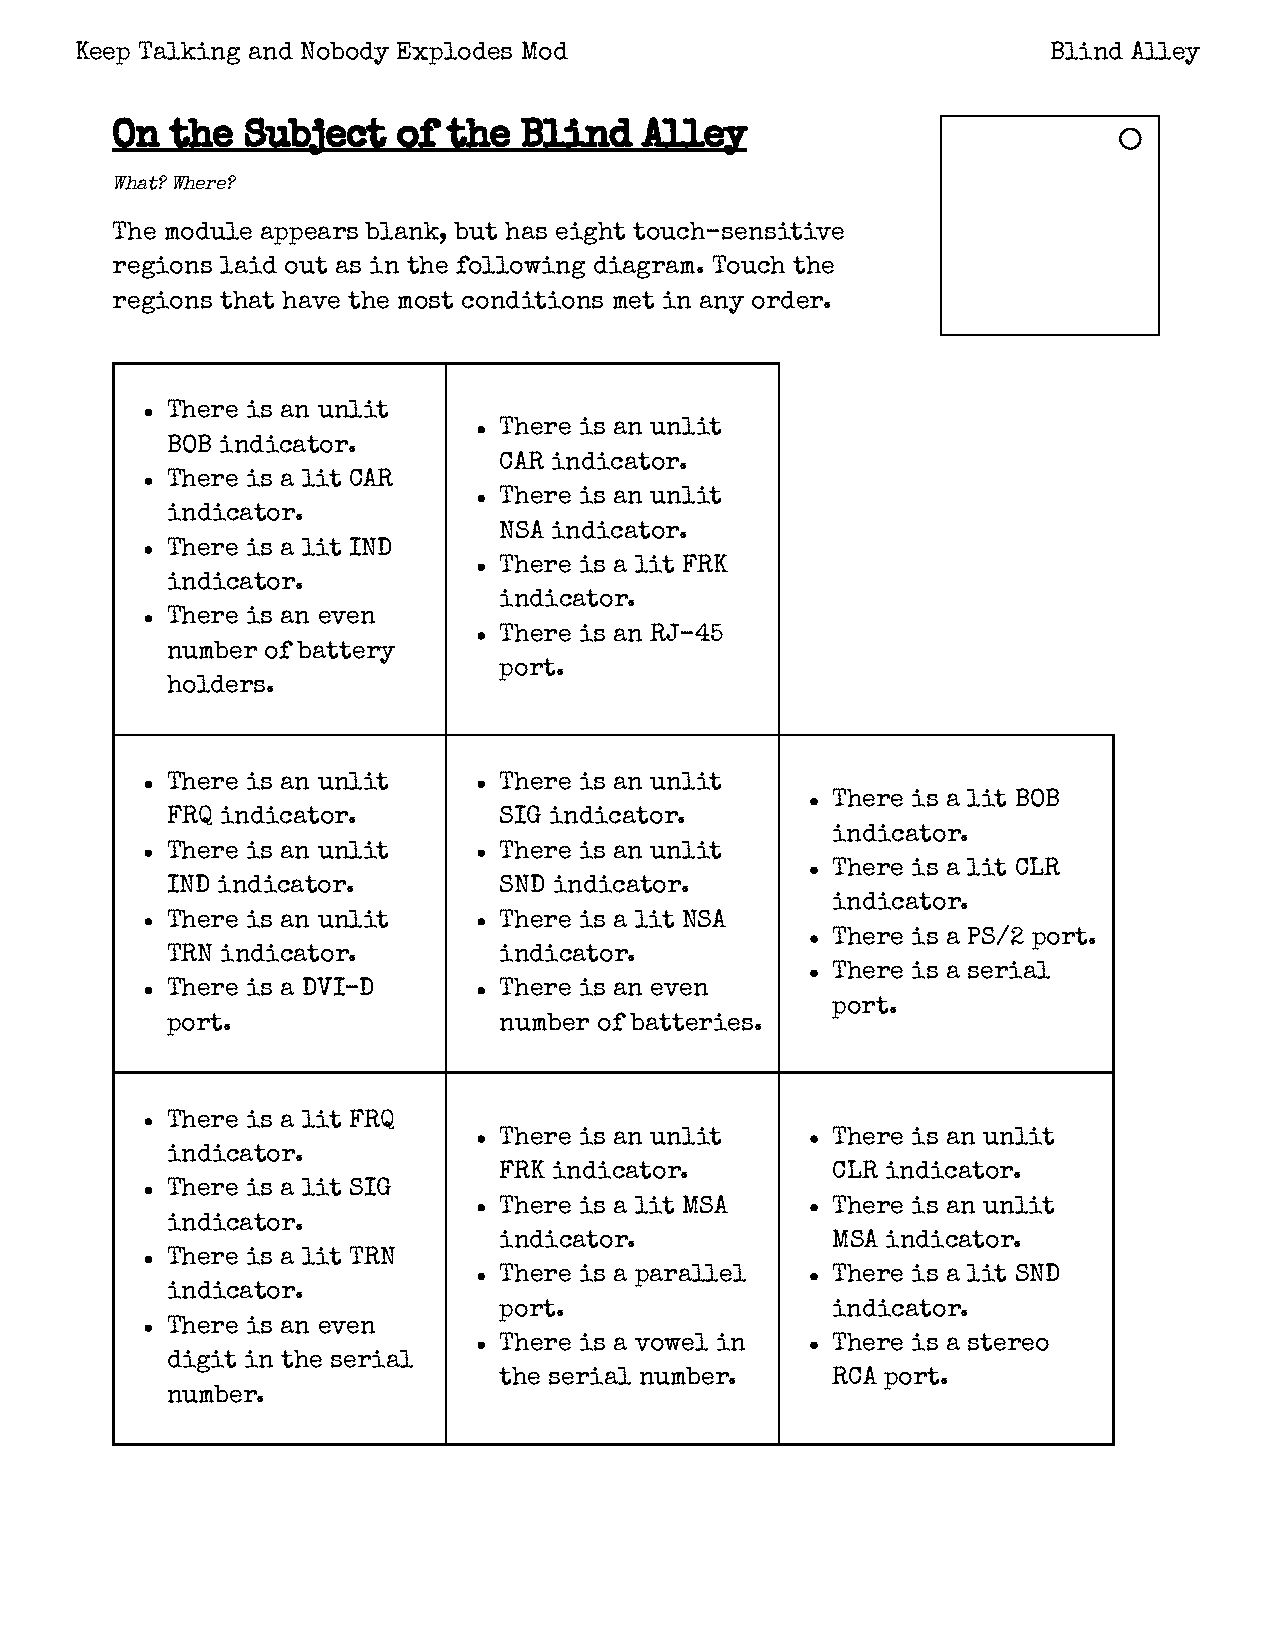
\includepdf[pages=-,pagecommand={}]{pdf/timing/BlindAlley.pdf}

\newpage
\vspace*{-4cm}
\centerline{
\begin{overpic}[scale=1.0,unit=1mm,page=1]{pdf/timing/TurnTheKey.pdf}
    \put(160,20){
\includegraphics{attention.png}}
\end{overpic}
}

\newpage
 
\includepdf[pages=2,pagecommand={}]{pdf/timing/TurnTheKey.pdf}

\invisiblesection{Wires, Electronics}
 \includepdf[scale=0.9,pages=5,pagecommand={}]{pdf/sections.pdf}

\newpage
\thispagestyle{empty}
\mbox{}

\newpage
\vspace*{-4cm}
\centerline{
\begin{overpic}[scale=1.0,unit=1mm,page=5]{pdf/vanilla.pdf}
    \put(160,20){
\includegraphics{attention.png}}
\end{overpic}
}


\newpage
 
\includepdf[pages=13,pagecommand={}]{pdf/vanilla.pdf}

\newpage
\vspace*{-4cm}
\centerline{
\begin{overpic}[scale=1.0,unit=1mm,page=14]{pdf/vanilla.pdf}
    \put(165,20){
\includegraphics{attention.png}}
\end{overpic}
}

\newpage
 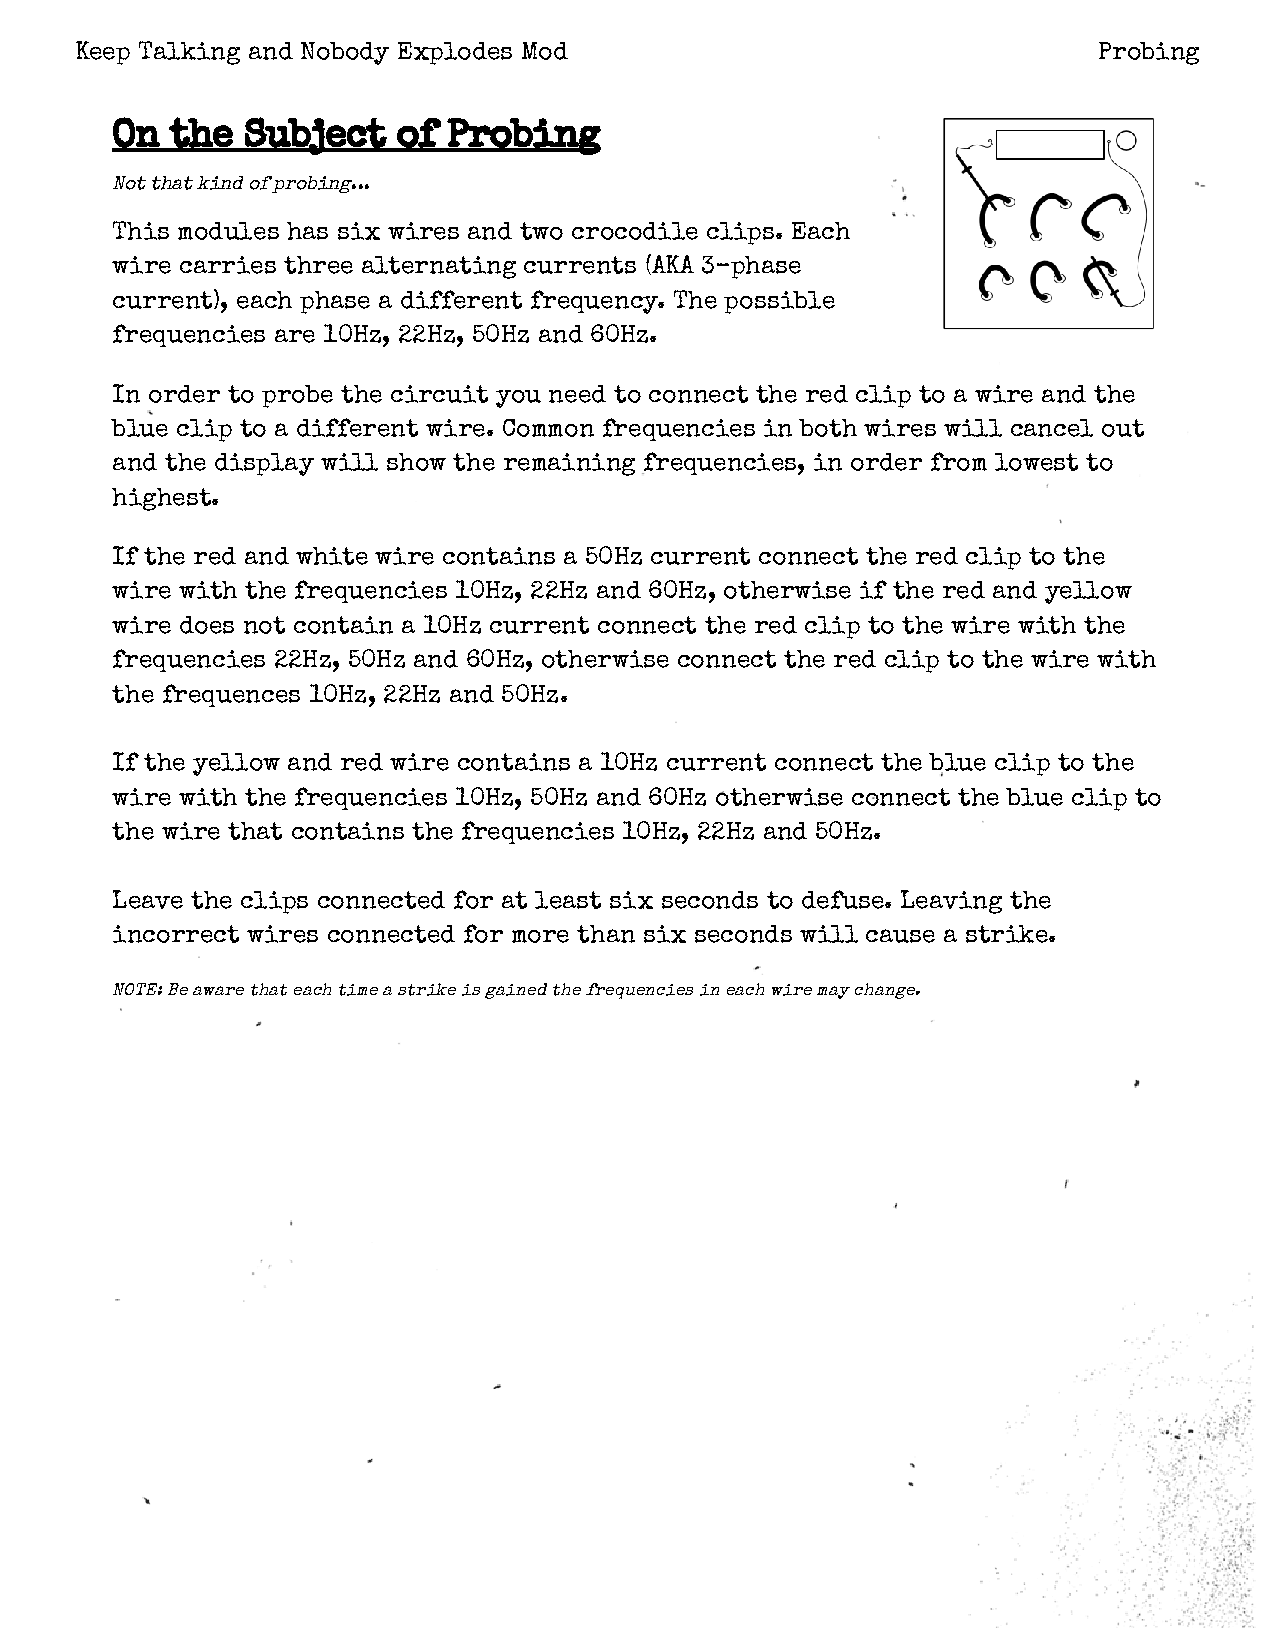
\includepdf[pages=-,pagecommand={}]{pdf/electronics/Probing.pdf}

\newpage
 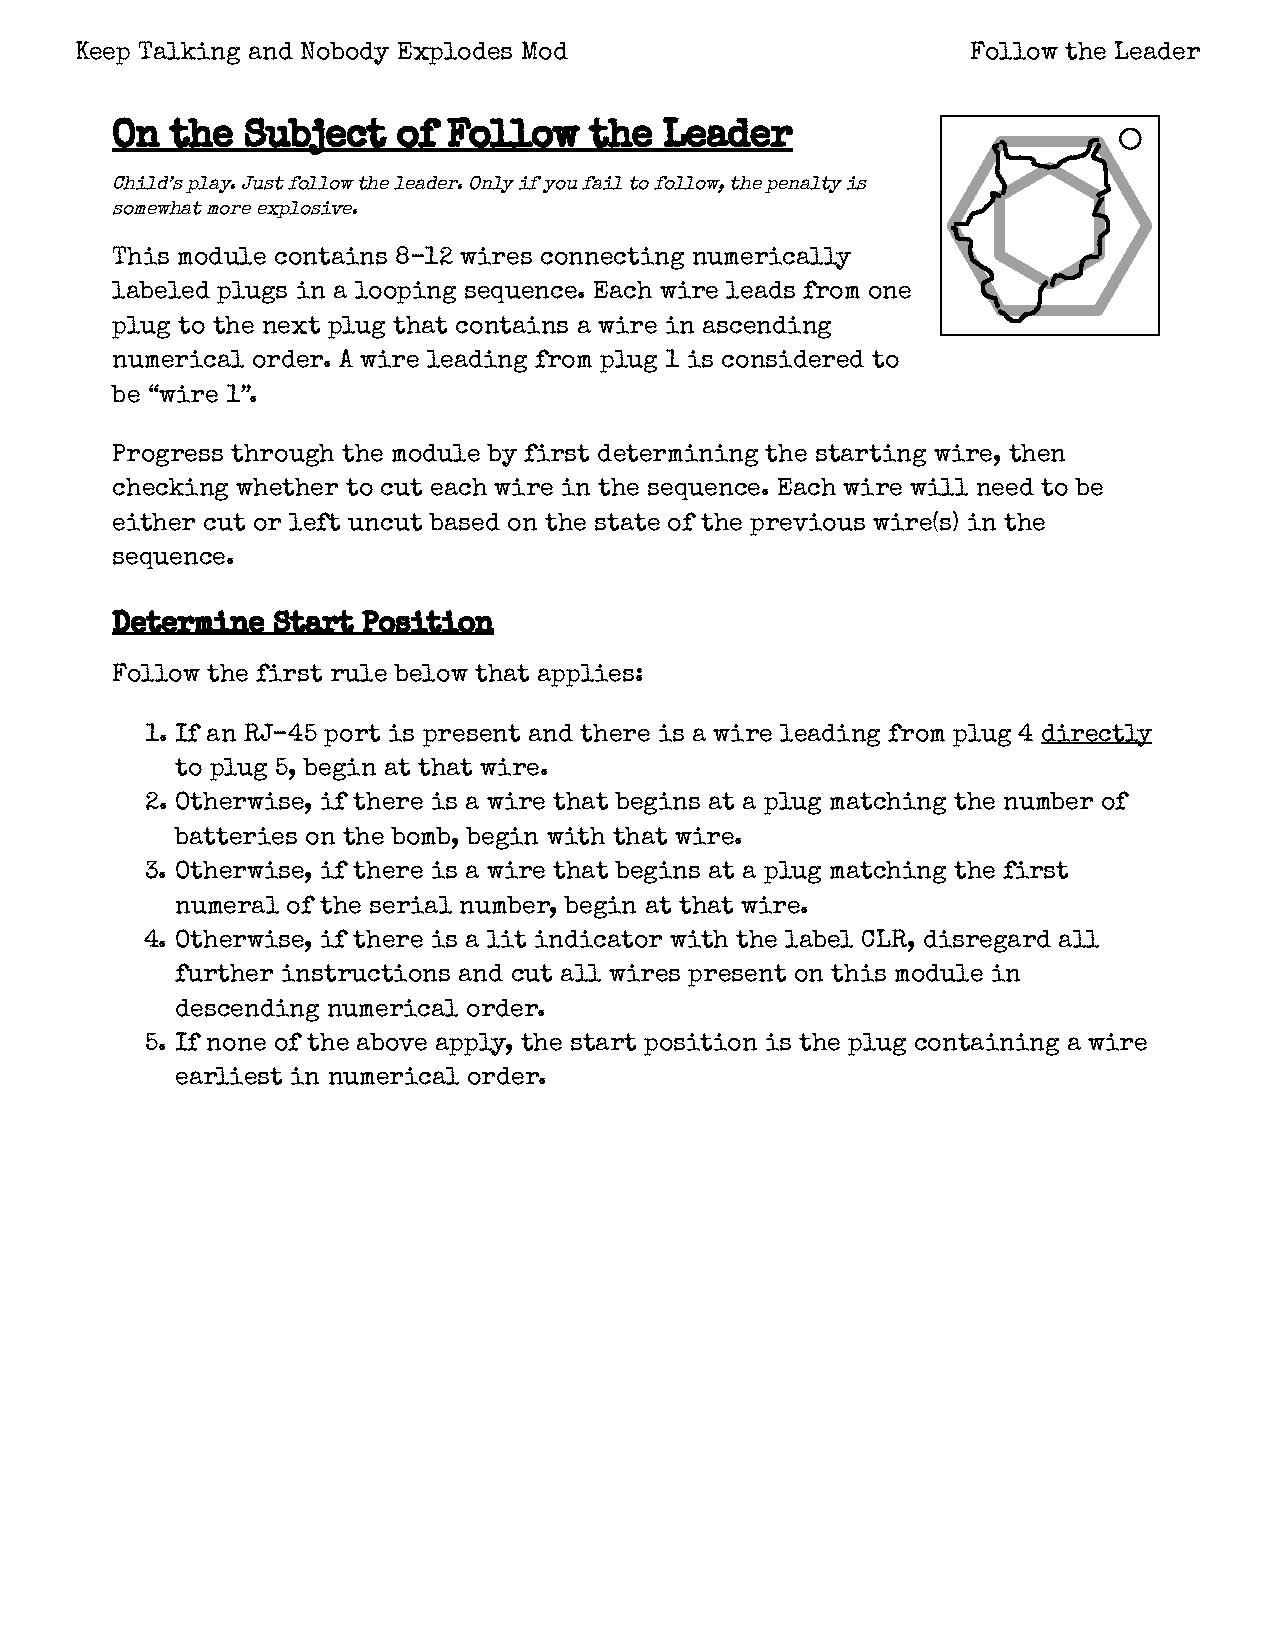
\includepdf[scale=1,pages=-,pagecommand={}]{pdf/electronics/FollowTheLeader.pdf}

\newpage
 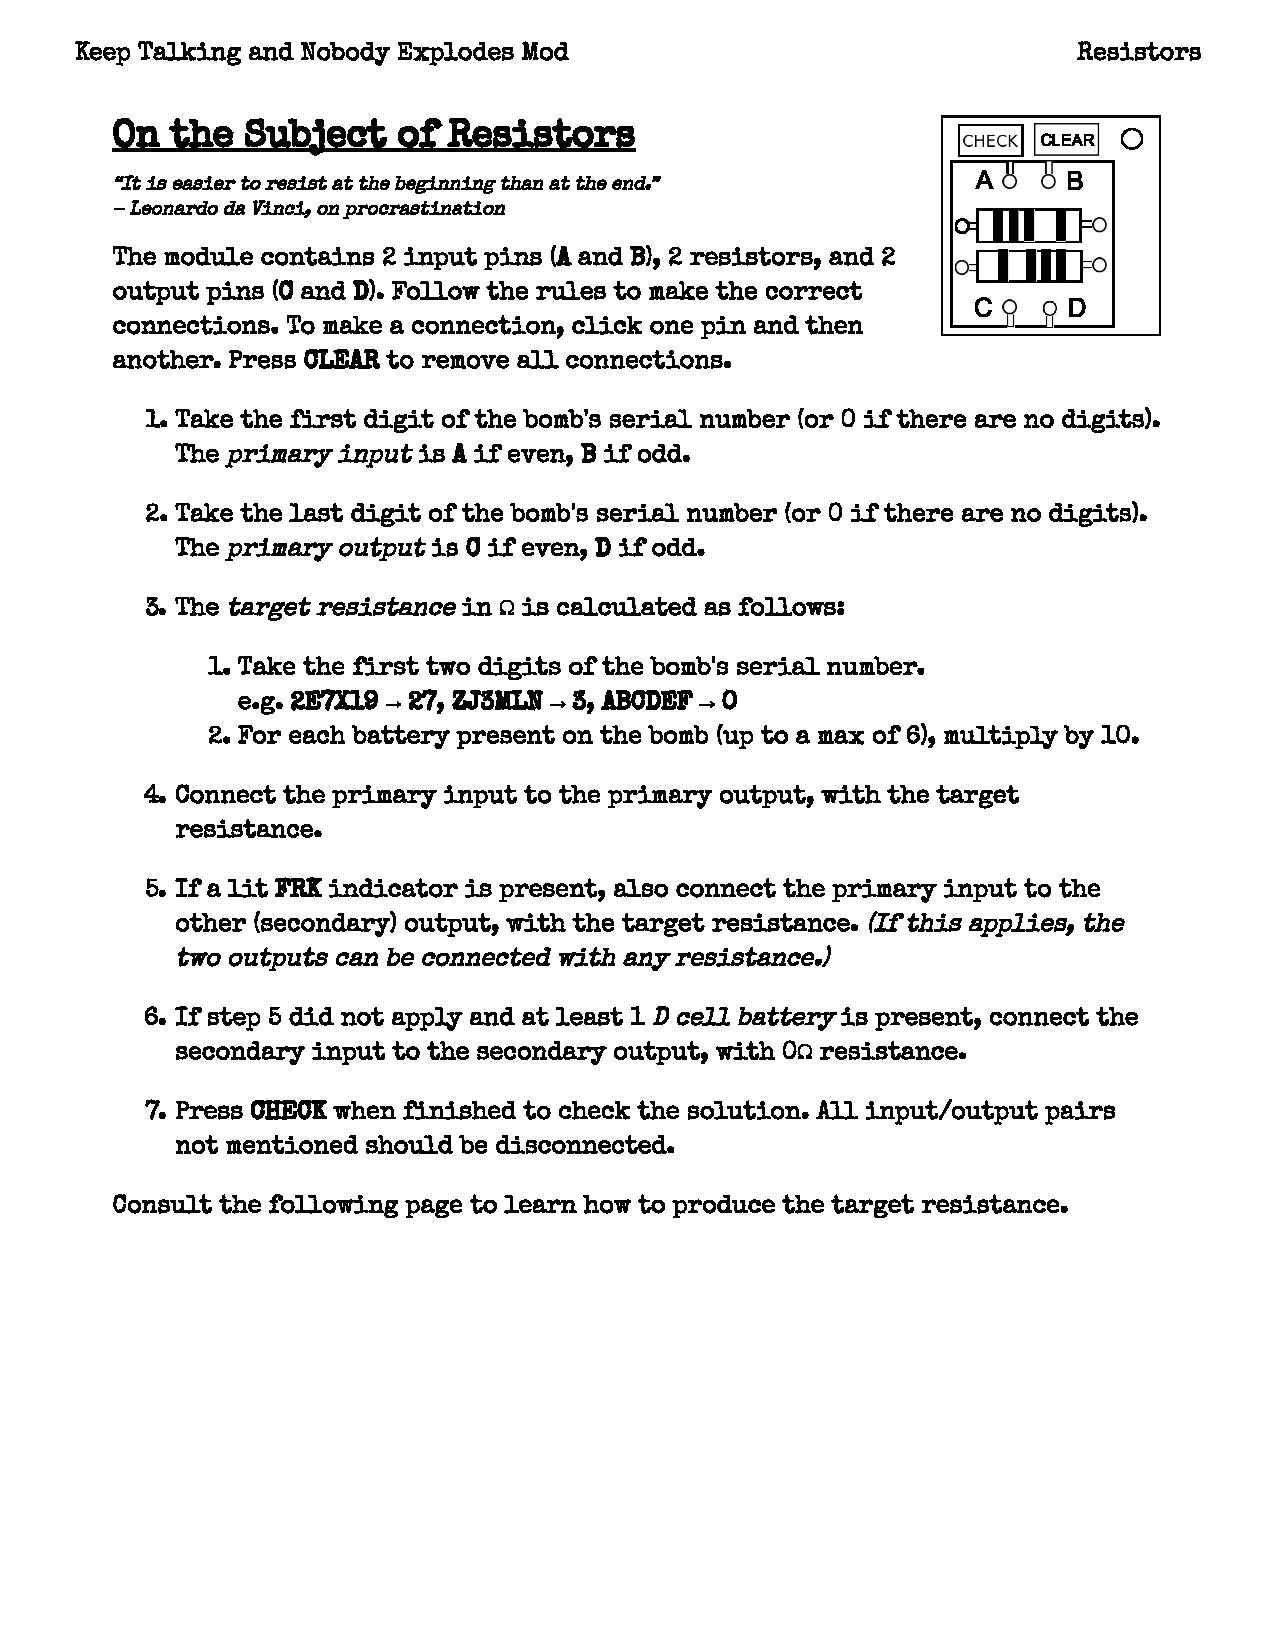
\includepdf[scale=1,pages=-,pagecommand={}]{pdf/electronics/resistors.pdf}

\newpage
 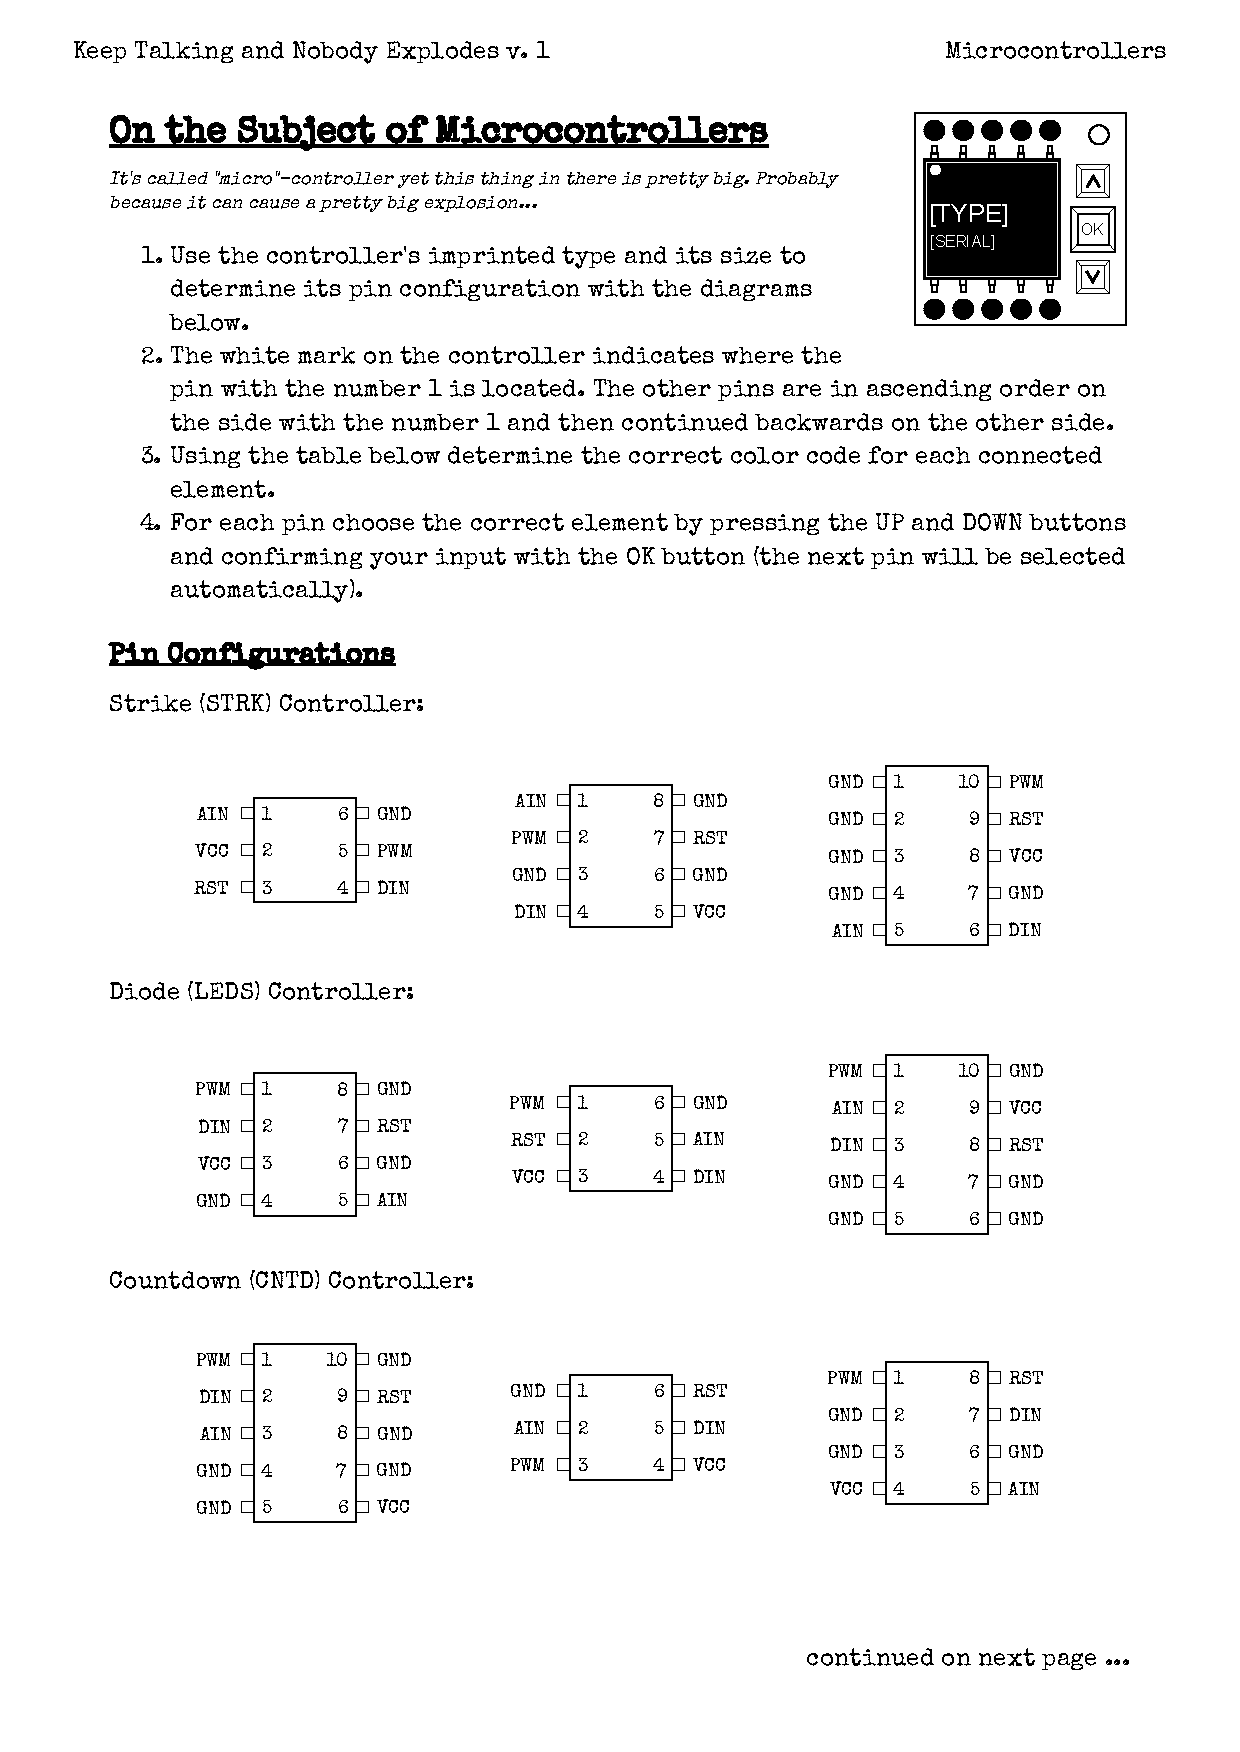
\includepdf[scale=1,pages=-,pagecommand={}]{pdf/electronics/microcontroller.pdf}

\newpage
\invisiblesection{Four symmetrical Buttons}
 \includepdf[scale=1,pages=6,pagecommand={}]{pdf/sections.pdf}


\newpage
\thispagestyle{empty}
\mbox{}


\newpage
\vspace*{-4cm}
\centerline{
\begin{overpic}[scale=1.0,page=7,unit=1mm]{pdf/vanilla.pdf}
    \put(160,20){
\includegraphics{attention.png}}
\end{overpic}
}

\newpage
 
\includepdf[scale=1,pages=15,pagecommand={}]{pdf/vanilla.pdf}


\newpage
\vspace*{-4cm}
\centerline{
\begin{overpic}[scale=1.0,unit=1mm]{pdf/4buttons/alphabet.pdf}
    \put(160,20){
\includegraphics{attention.png}}
\end{overpic}
}

\newpage
 
\includepdf[pages=-,pagecommand={}]{pdf/4buttons/LetteredKeys.pdf}

\newpage
\vspace*{-4cm}
\centerline{
\begin{overpic}[scale=1.0,unit=1mm,page=8]{pdf/vanilla.pdf}
    \put(160,20){
\includegraphics{attention.png}}
\end{overpic}
}


\newpage
 
\includepdf[pages=11,pagecommand={}]{pdf/vanilla.pdf}

\newpage

\includepdf[scale=0.9,pages=8-9,pagecommand={}]{pdf/advanced.pdf}

\newpage
 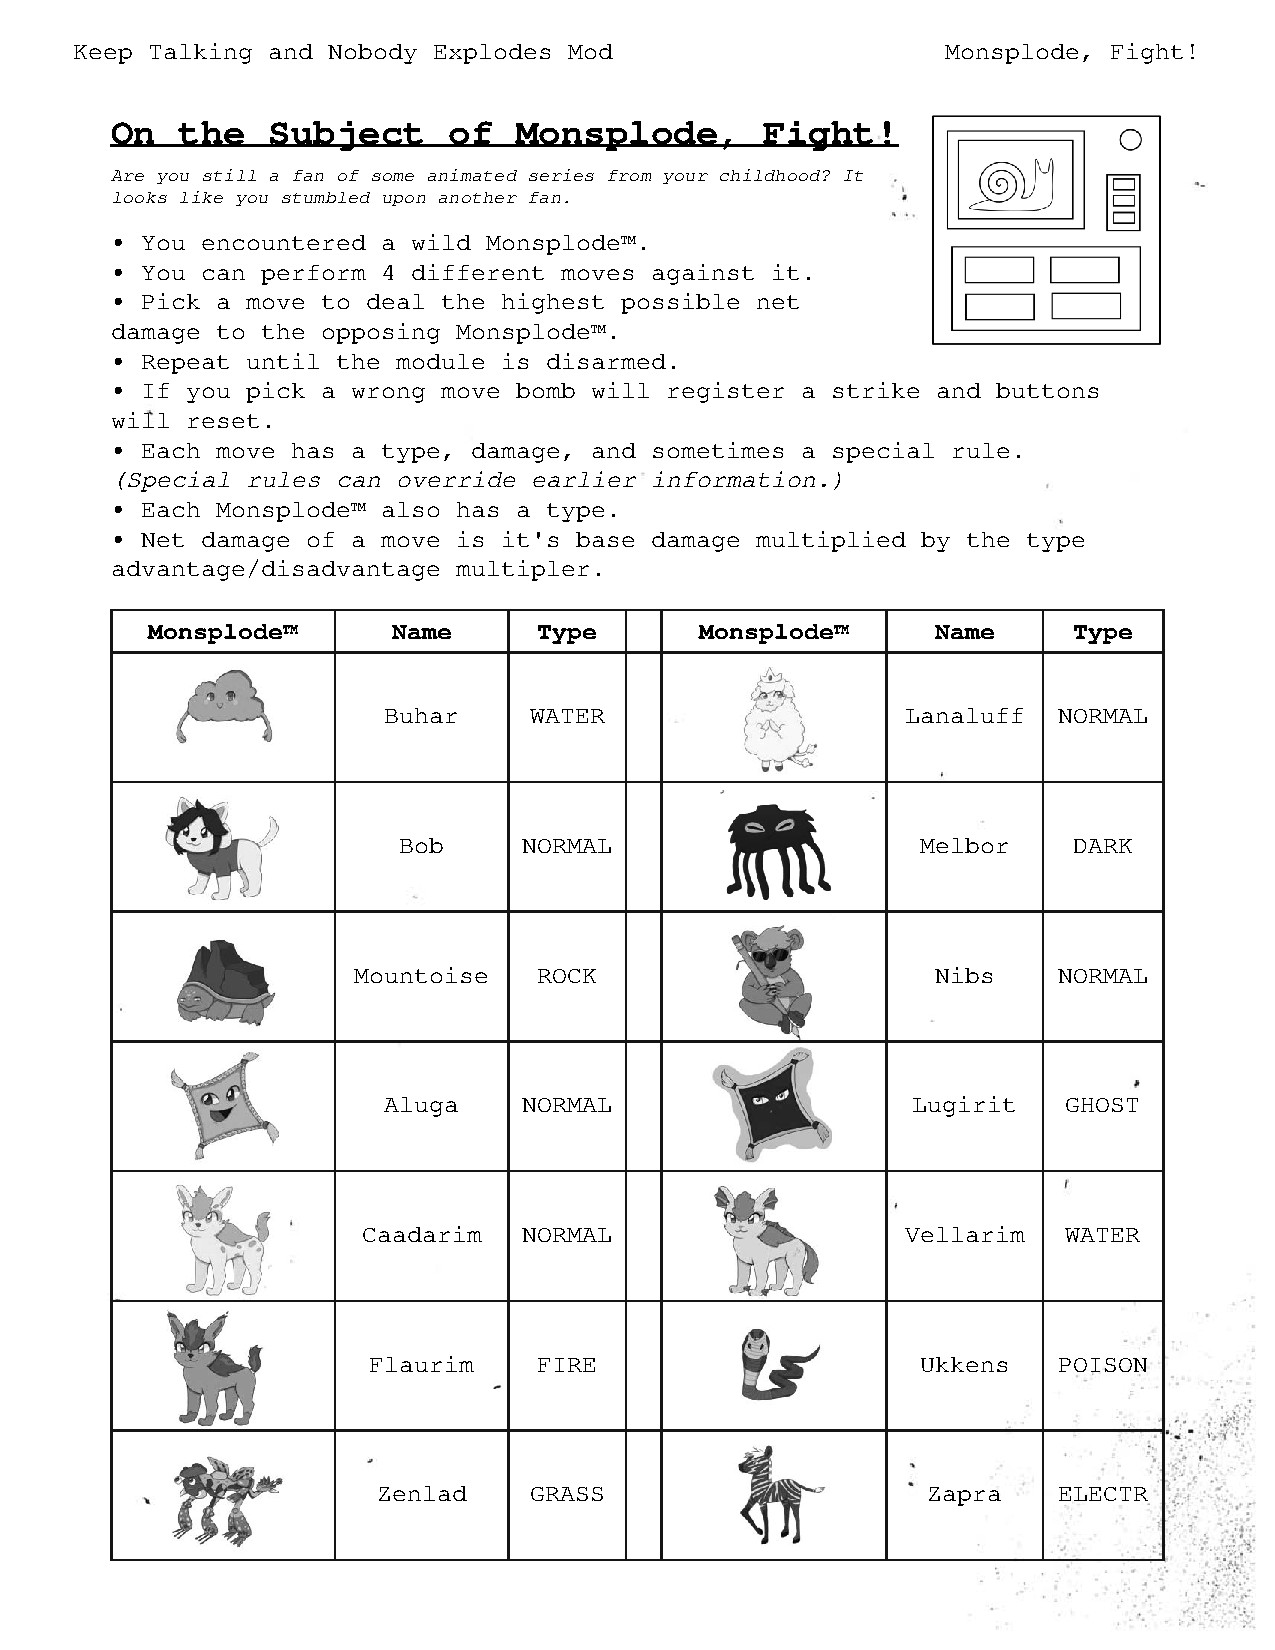
\includepdf[scale=0.9,pages=-,pagecommand={}]{pdf/4buttons/MonsplodeFightManual.pdf}

\newpage
\thispagestyle{empty}
\mbox{}

\invisiblesection{More than six Buttons}
\includepdf[pages=7,pagecommand={}]{pdf/sections.pdf}

\newpage
\thispagestyle{empty}
\mbox{}

\newpage
\vspace*{-4cm}
\centerline{
\begin{overpic}[scale=1.0,unit=1mm]{pdf/6buttons/emojiMath.pdf}
    \put(160,20){
\includegraphics{attention.png}}
\end{overpic}
}

\newpage
 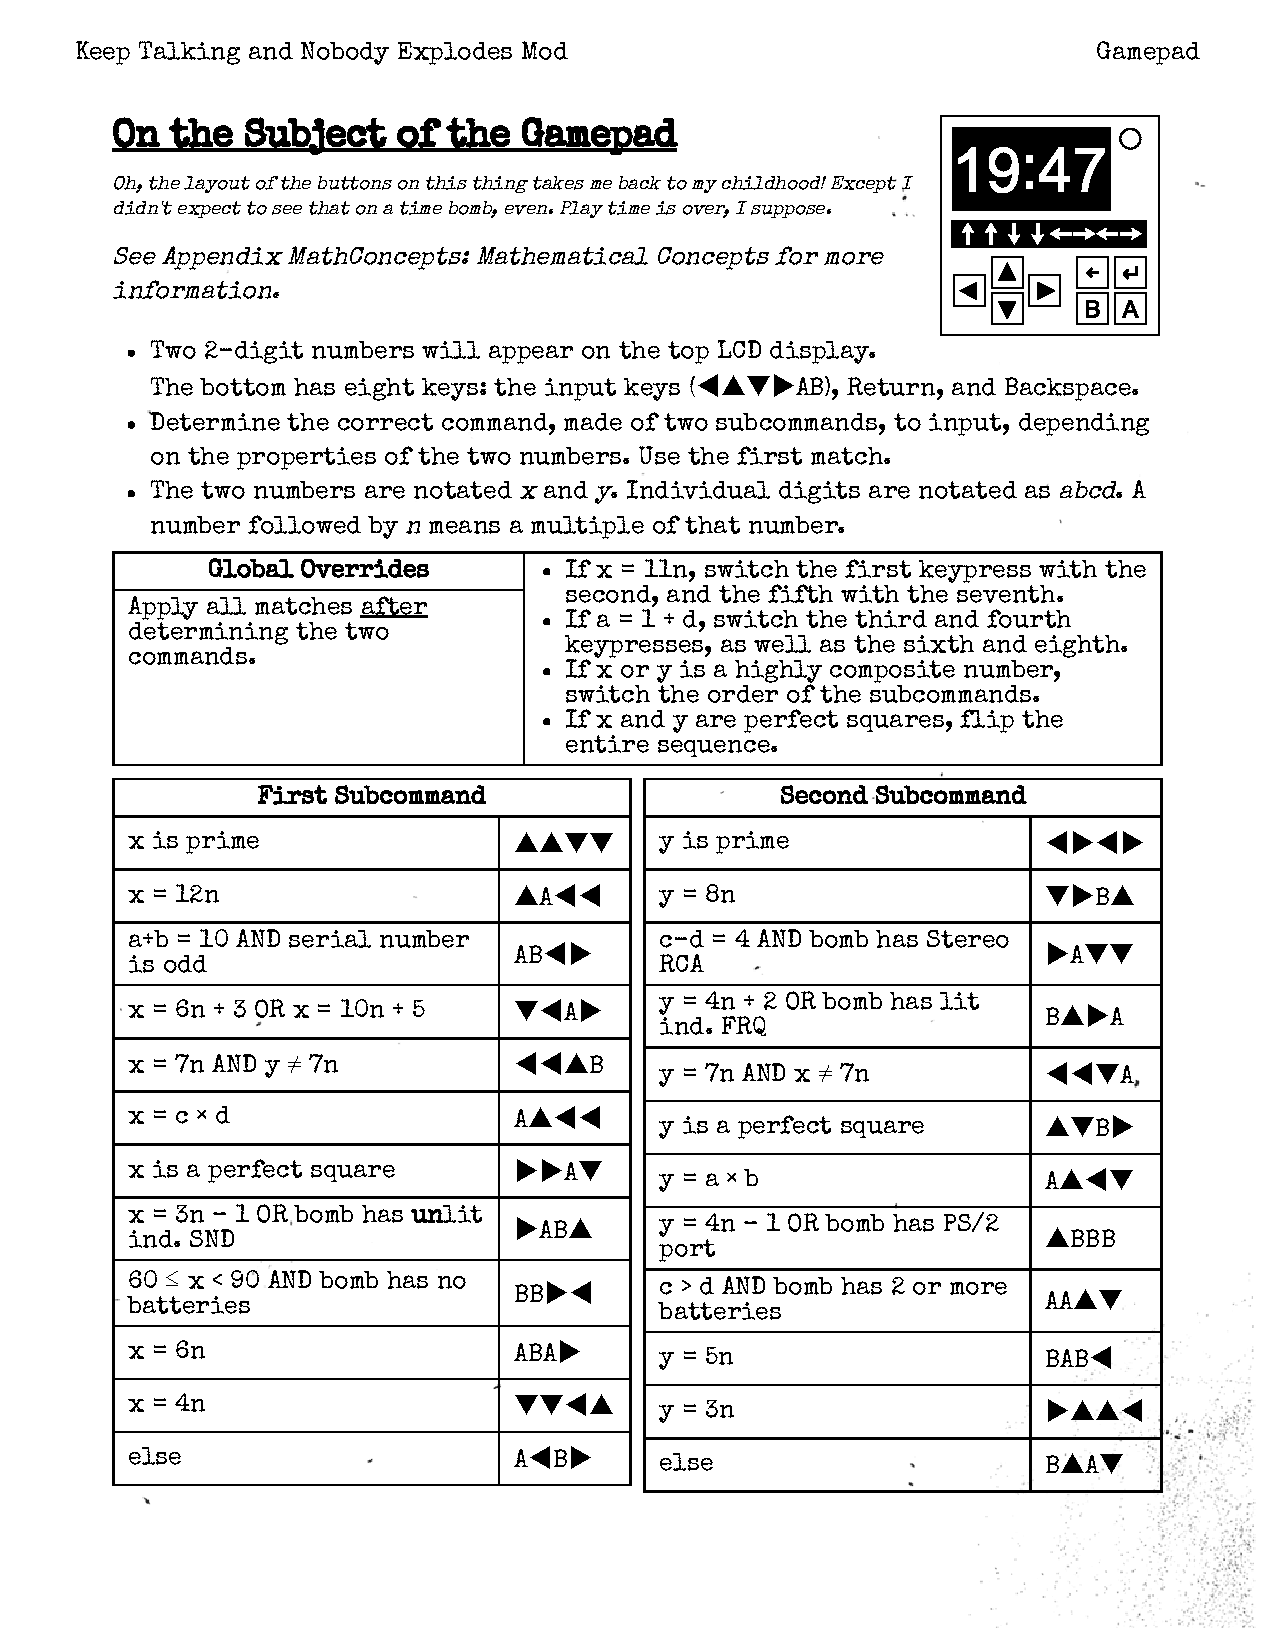
\includepdf[pages=1,pagecommand={}]{pdf/other/GamePad.pdf}

\newpage
 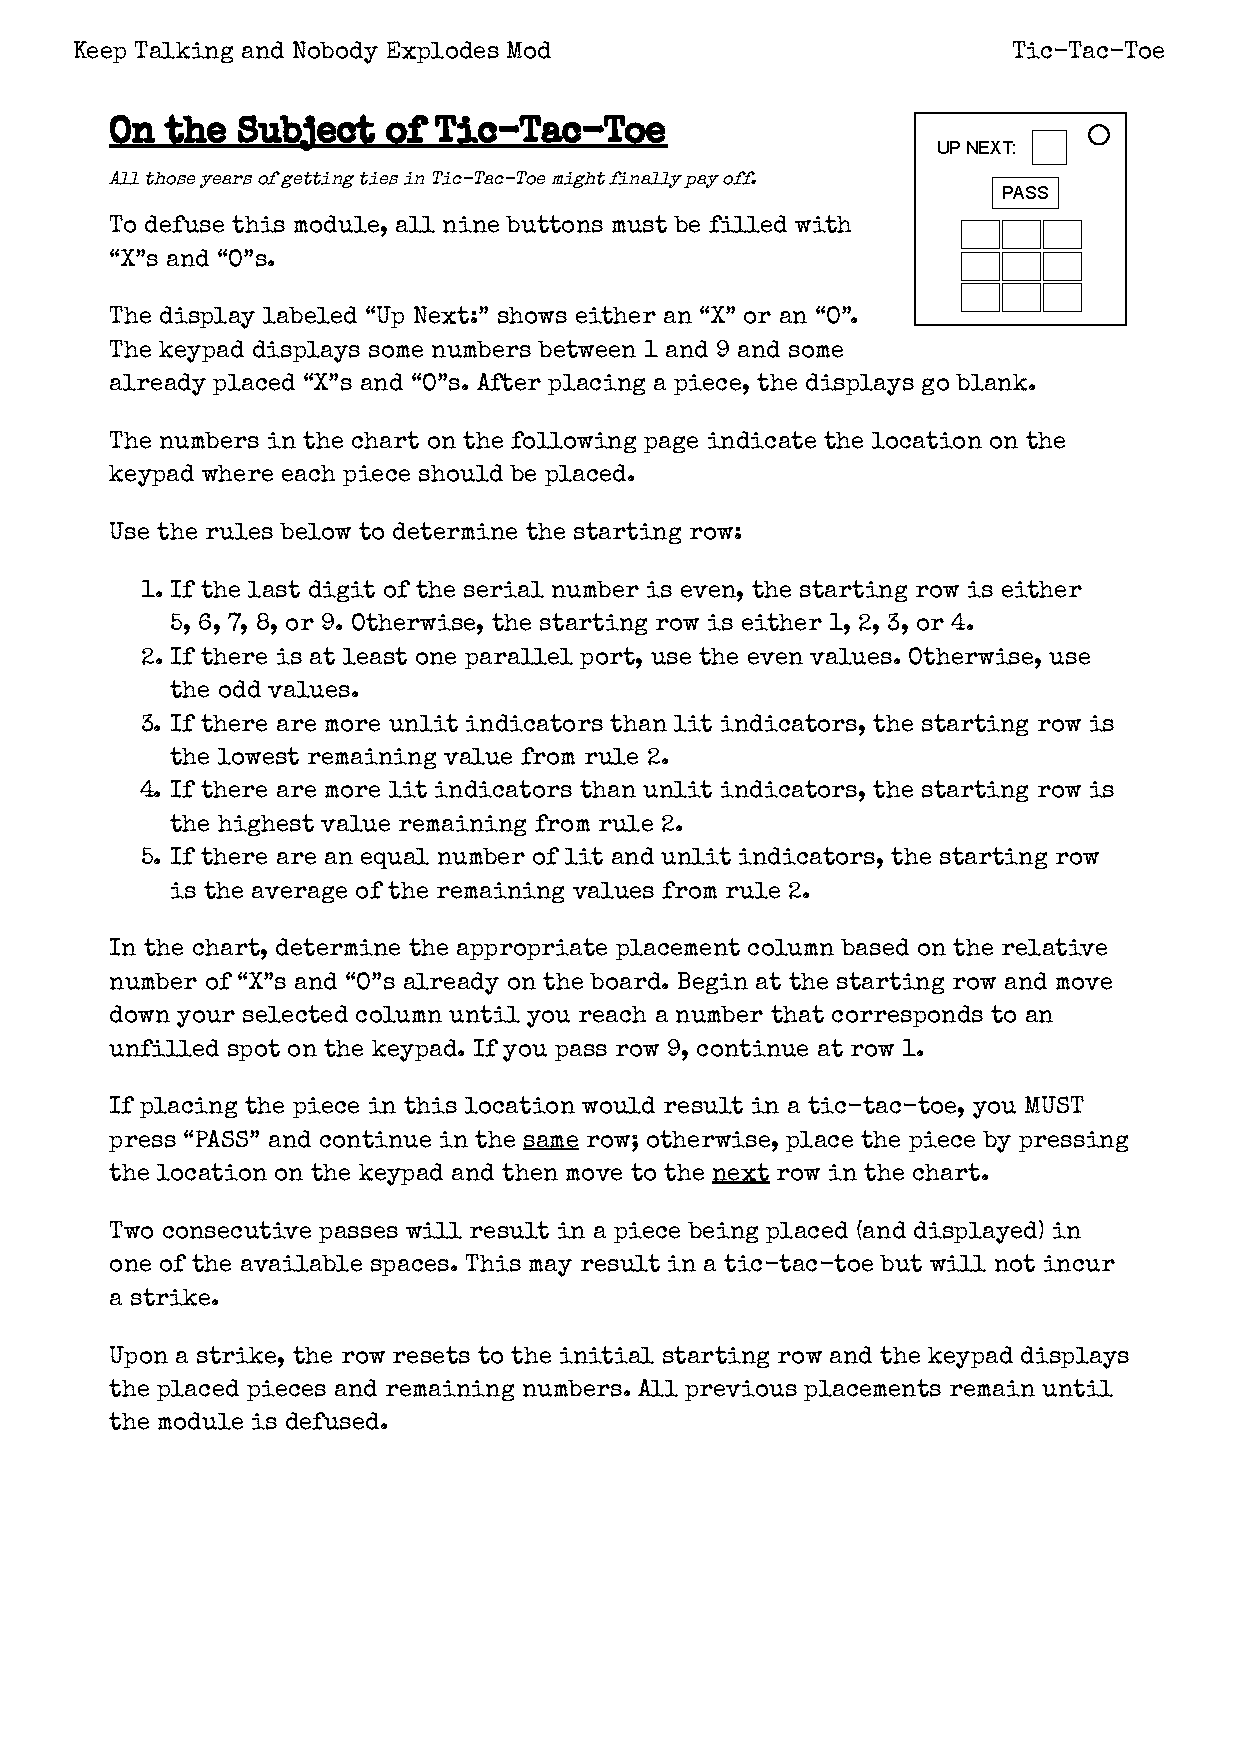
\includepdf[pages=-,pagecommand={}]{pdf/6buttons/TicTacToe.pdf}

\newpage
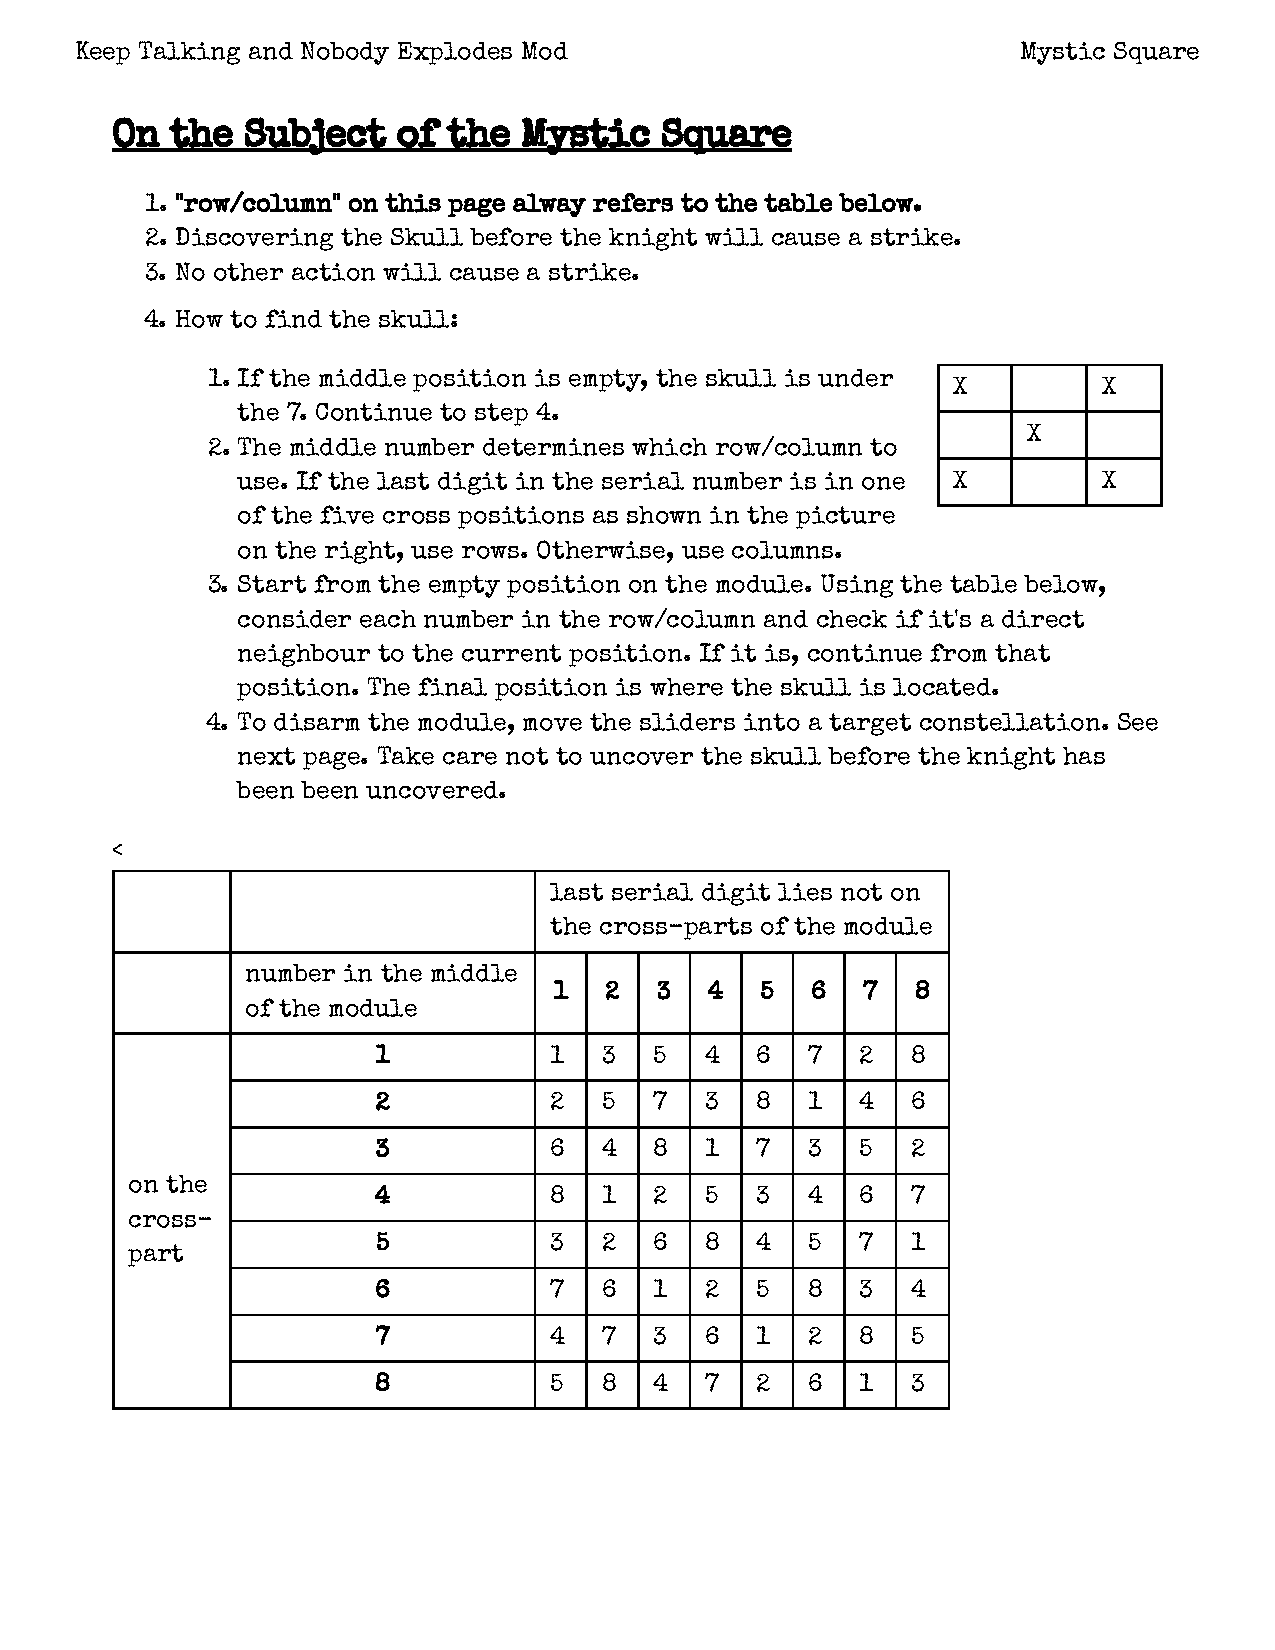
\includepdf[pages=-,pagecommand={}]{pdf/6buttons/SlidingPuzzle01.pdf}

\newpage
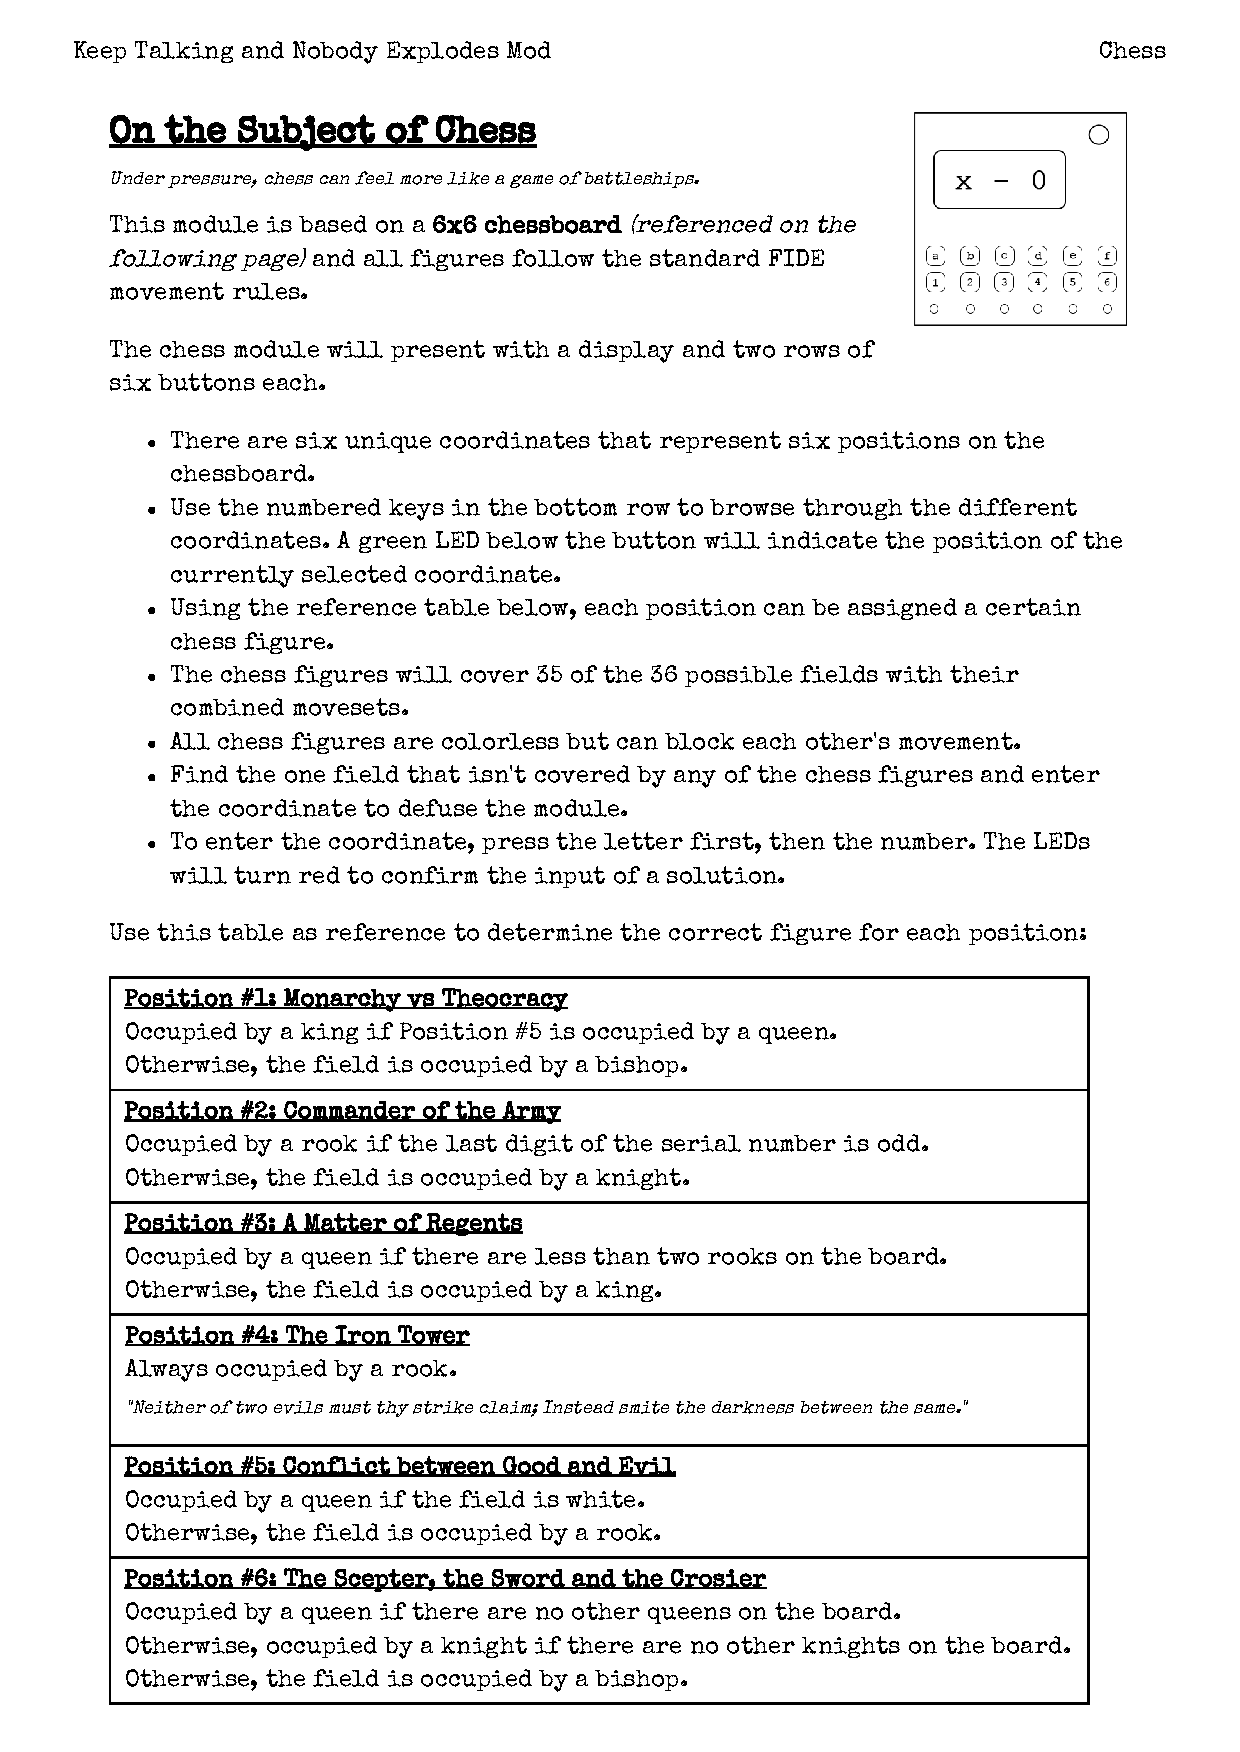
\includepdf[scale=0.9,pages=-,pagecommand={}]{pdf/6buttons/ChessModule.pdf}

\newpage
\vspace*{-4cm}
\centerline{
\begin{overpic}[scale=1.0,unit=1mm,page=1]{pdf/advanced.pdf}
       \put(175,20){
\includegraphics{attention.png}}
\end{overpic}
}

\newpage
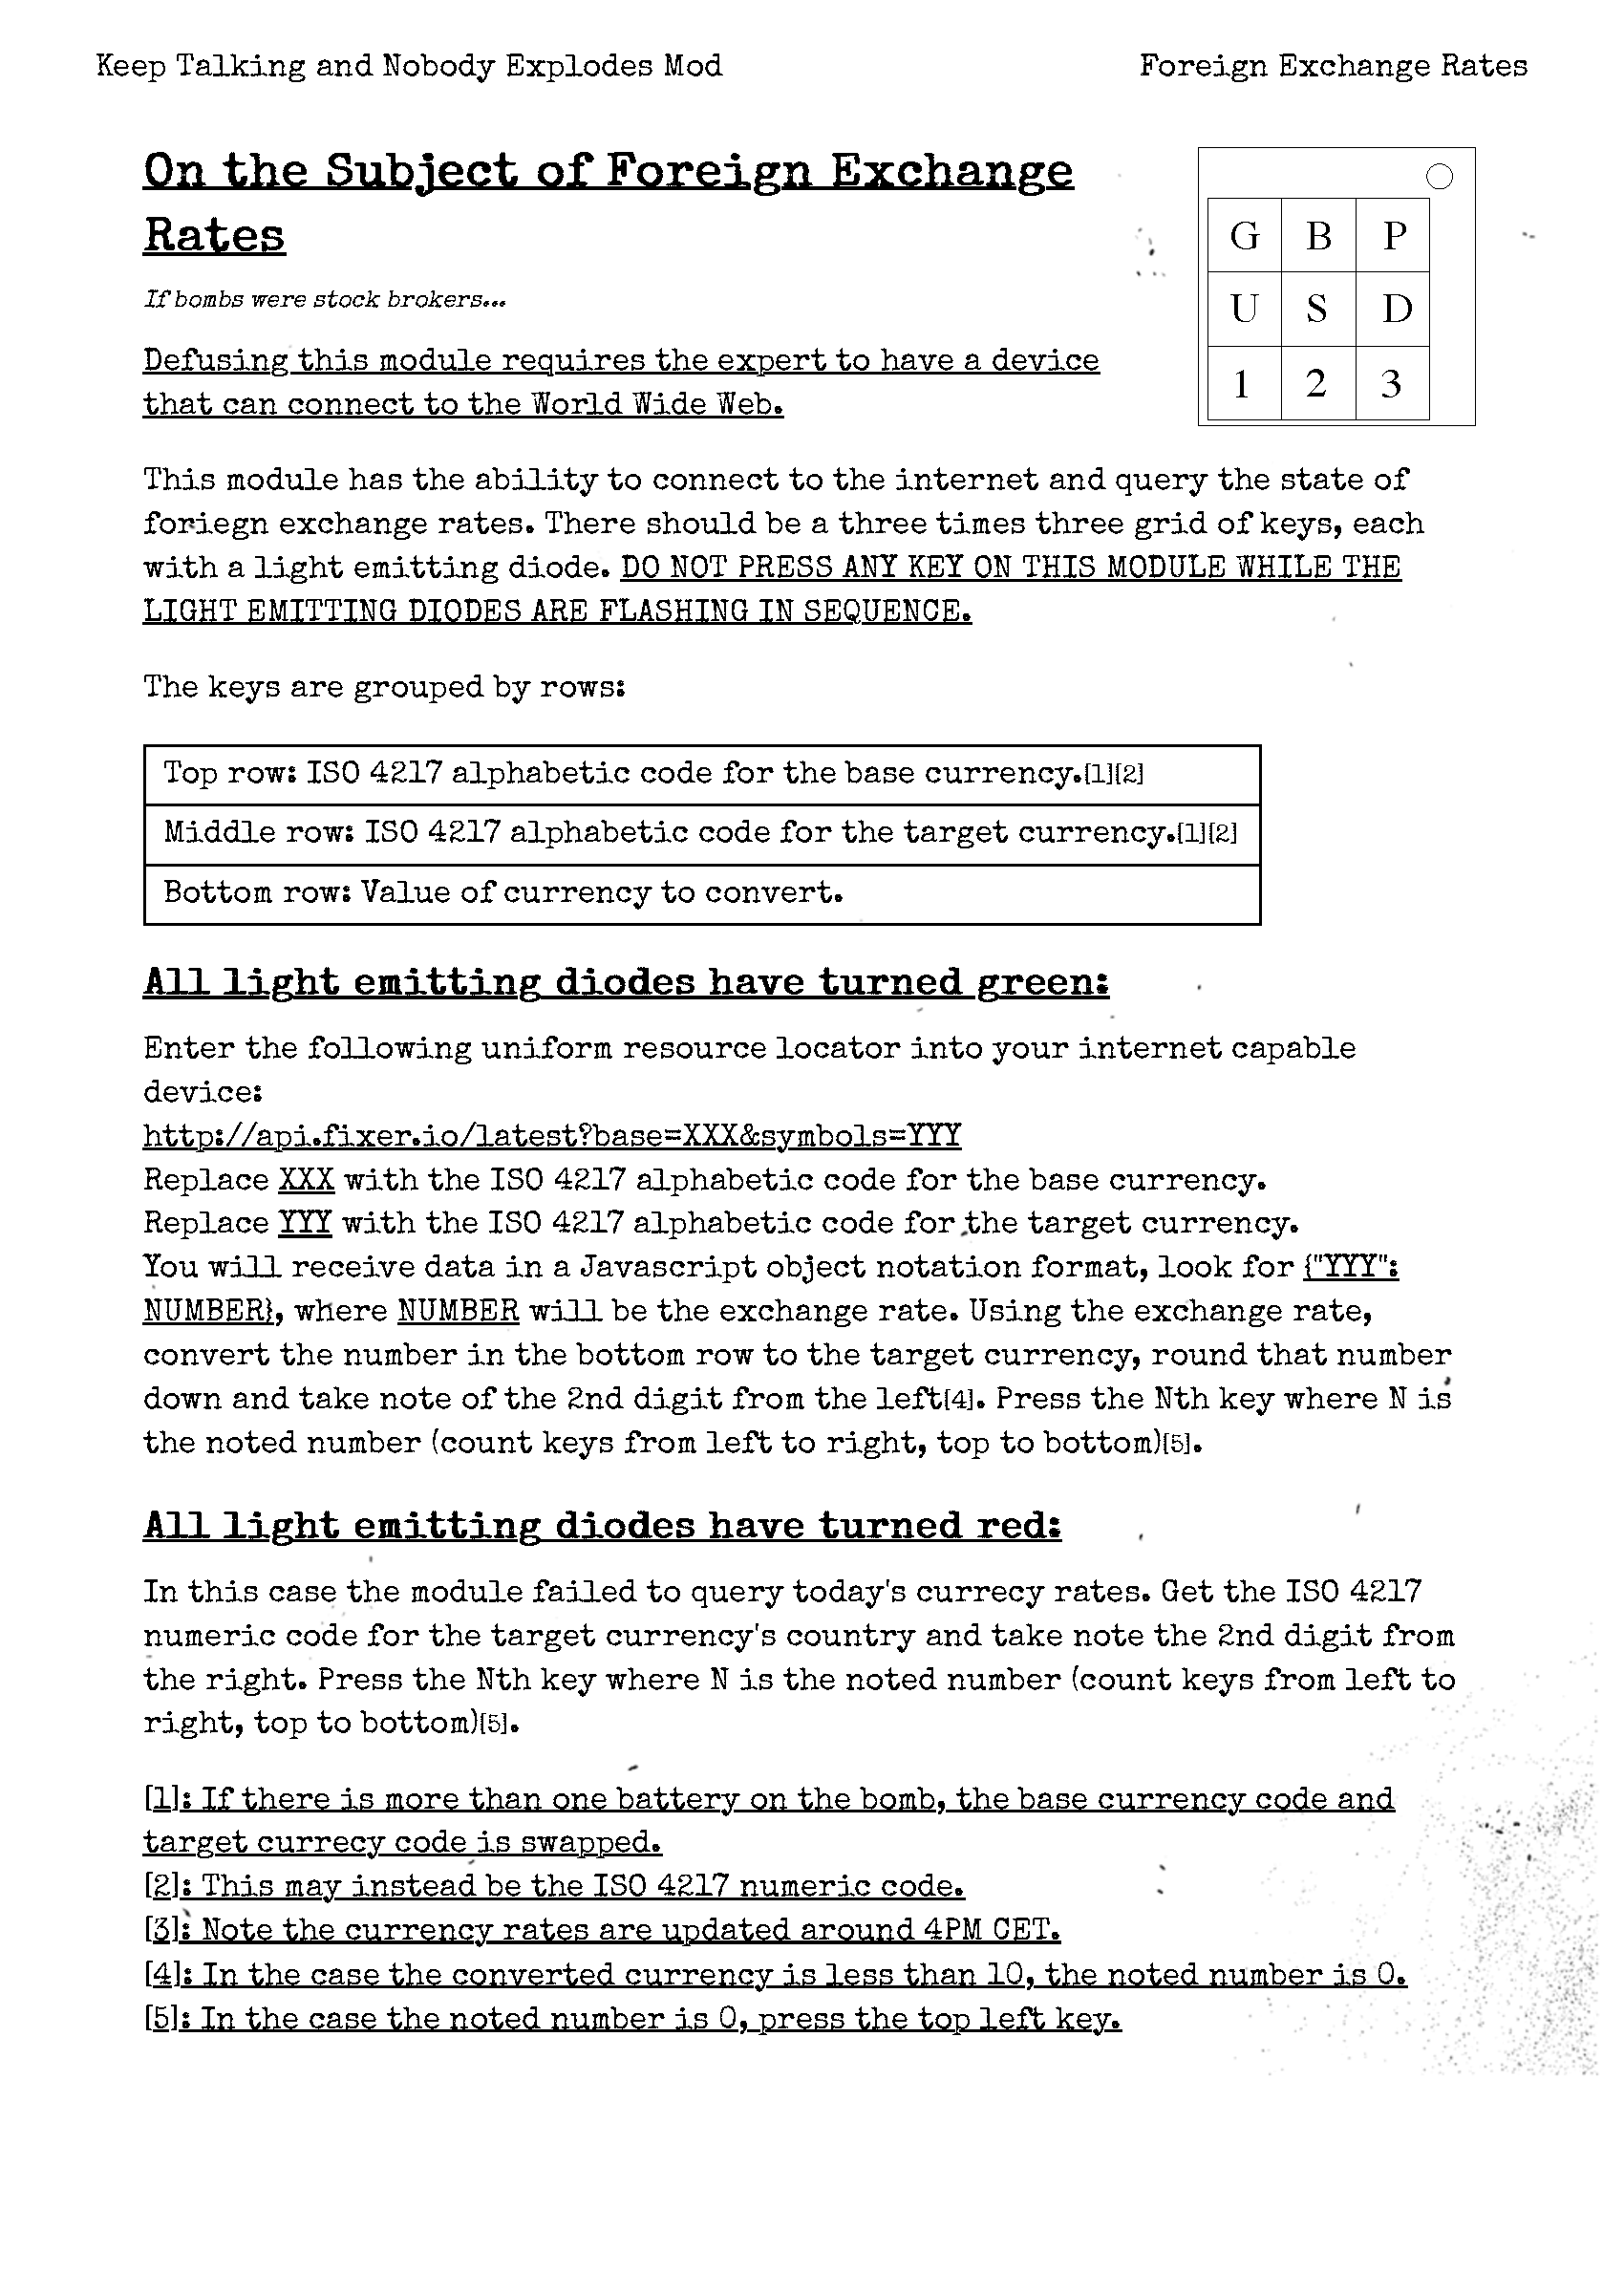
\includepdf[pages=-,pagecommand={}]{pdf/6buttons/ForeignExchangeRates.pdf}

\newpage
 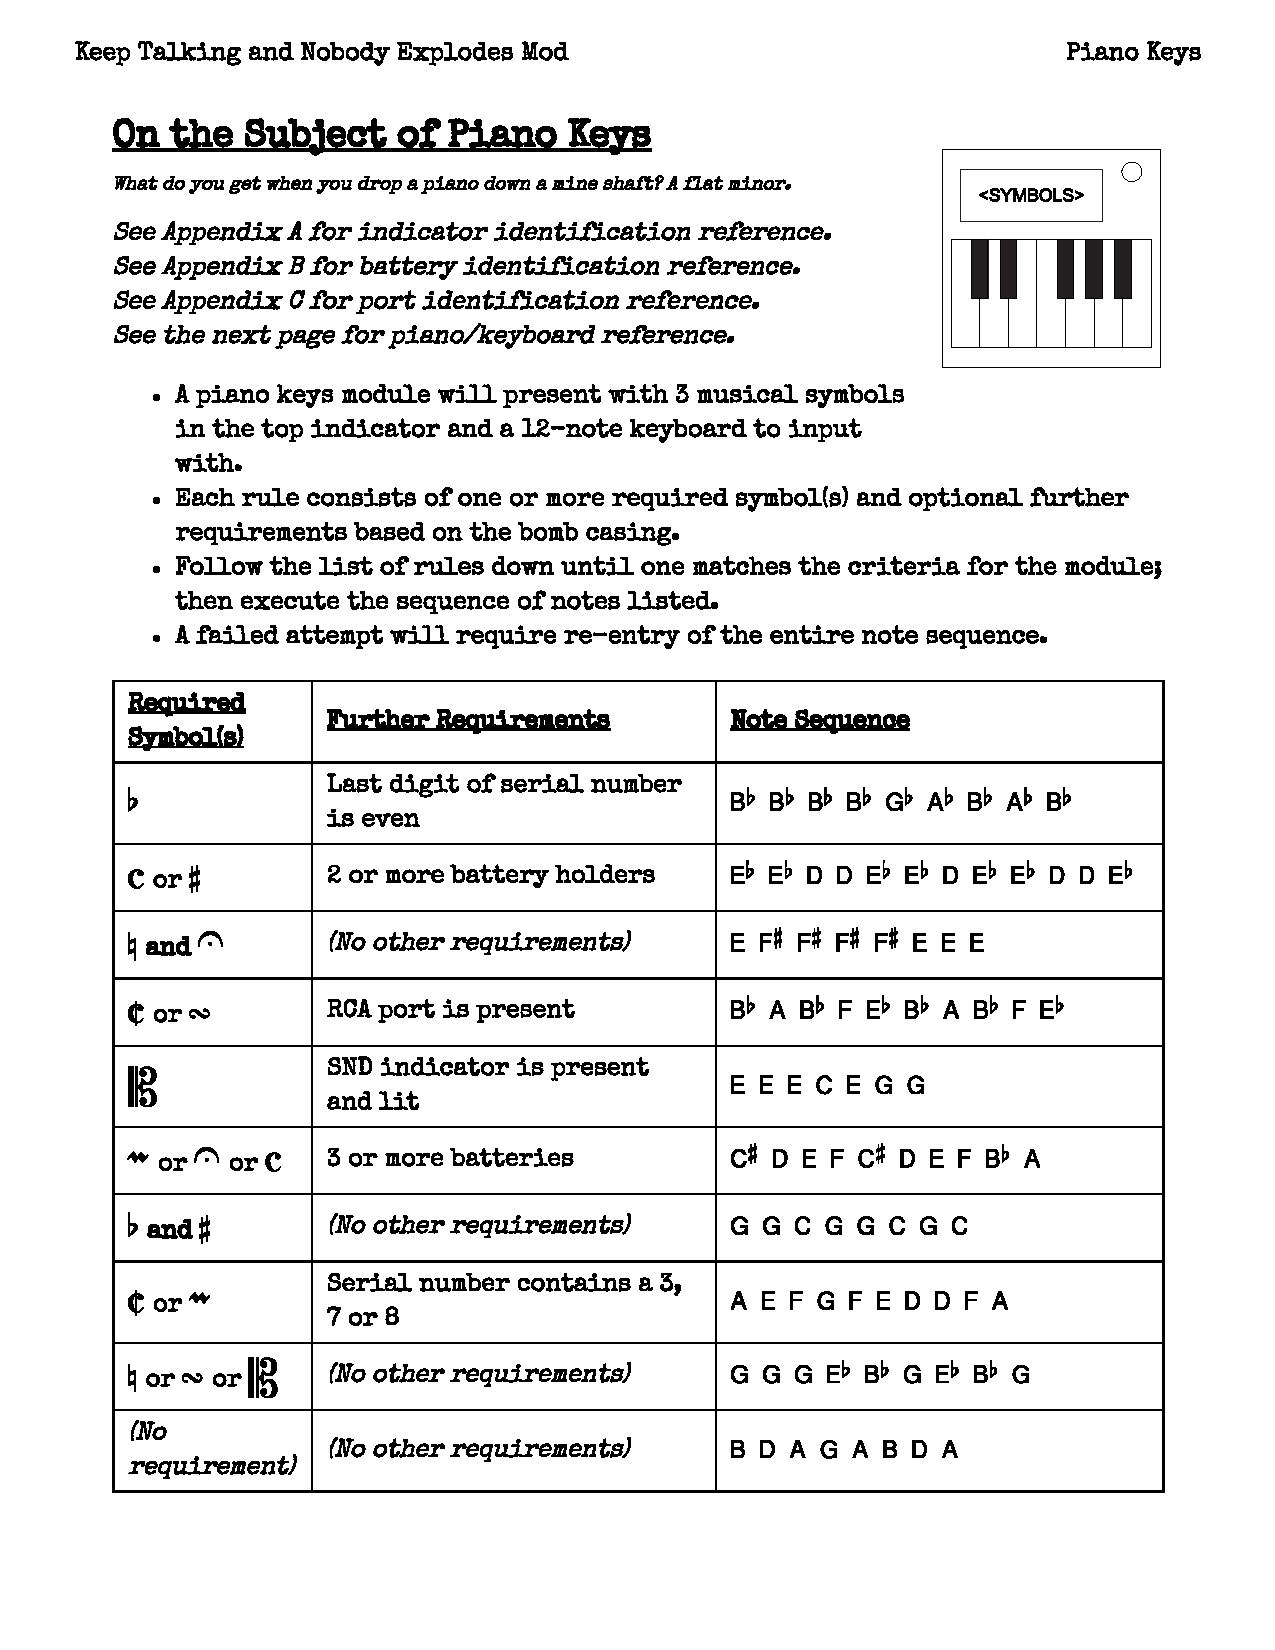
\includepdf[pages=-,pagecommand={}]{pdf/other/pianoKeys.pdf}

\newpage
\invisiblesection{Text}
\vspace*{-4cm}
\centerline{
\begin{overpic}[scale=0.9,unit=1mm,page=8]{pdf/sections.pdf}
\end{overpic}
}

\newpage
\thispagestyle{empty}
\mbox{}

\newpage
\vspace*{-4cm}
\centerline{
\begin{overpic}[scale=1.0,unit=1mm,page=1]{pdf/text/anagrams.pdf}
    \put(160,20){
\includegraphics{attention.png}}
\end{overpic}
}

\newpage
 
\includepdf[pages=2,pagecommand={}]{pdf/text/anagrams.pdf} 

\newpage
\vspace*{-4cm}
\centerline{
\begin{overpic}[scale=1.0,unit=1mm,page=1]{pdf/text/ceasarCipher.pdf}
    \put(160,20){
\includegraphics{attention.png}}
\end{overpic}
}

\newpage
 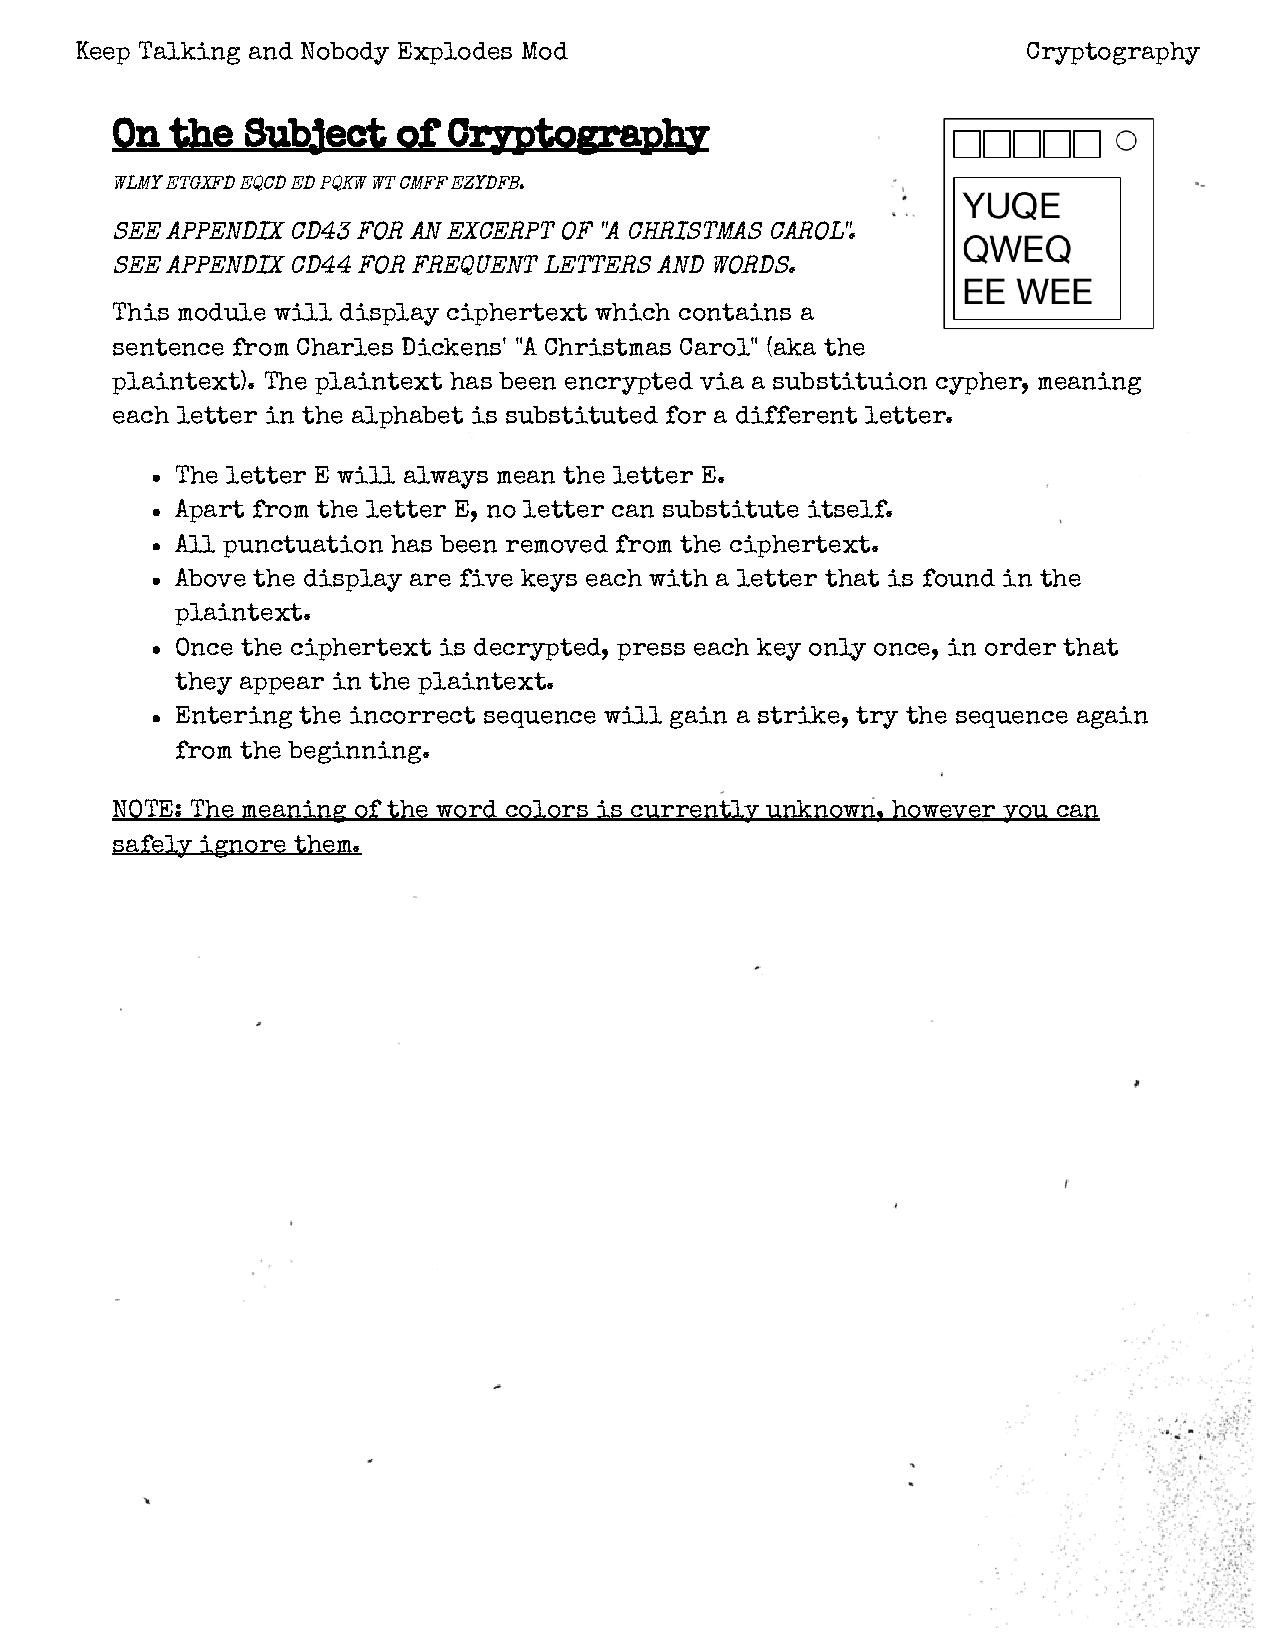
\includepdf[scale=1.0,pages=-,pagecommand={}]{pdf/text/Cryptography.pdf}

\newpage
 
\includepdf[pages=9-10,pagecommand={}]{pdf/vanilla.pdf}

\newpage
\vspace*{-4cm}
\centerline{
\begin{overpic}[scale=0.9,unit=1mm,page=1]{pdf/text/CrazyTalk.pdf}
    \put(160,20){
\includegraphics{attention.png}}
\end{overpic}
}

\newpage
 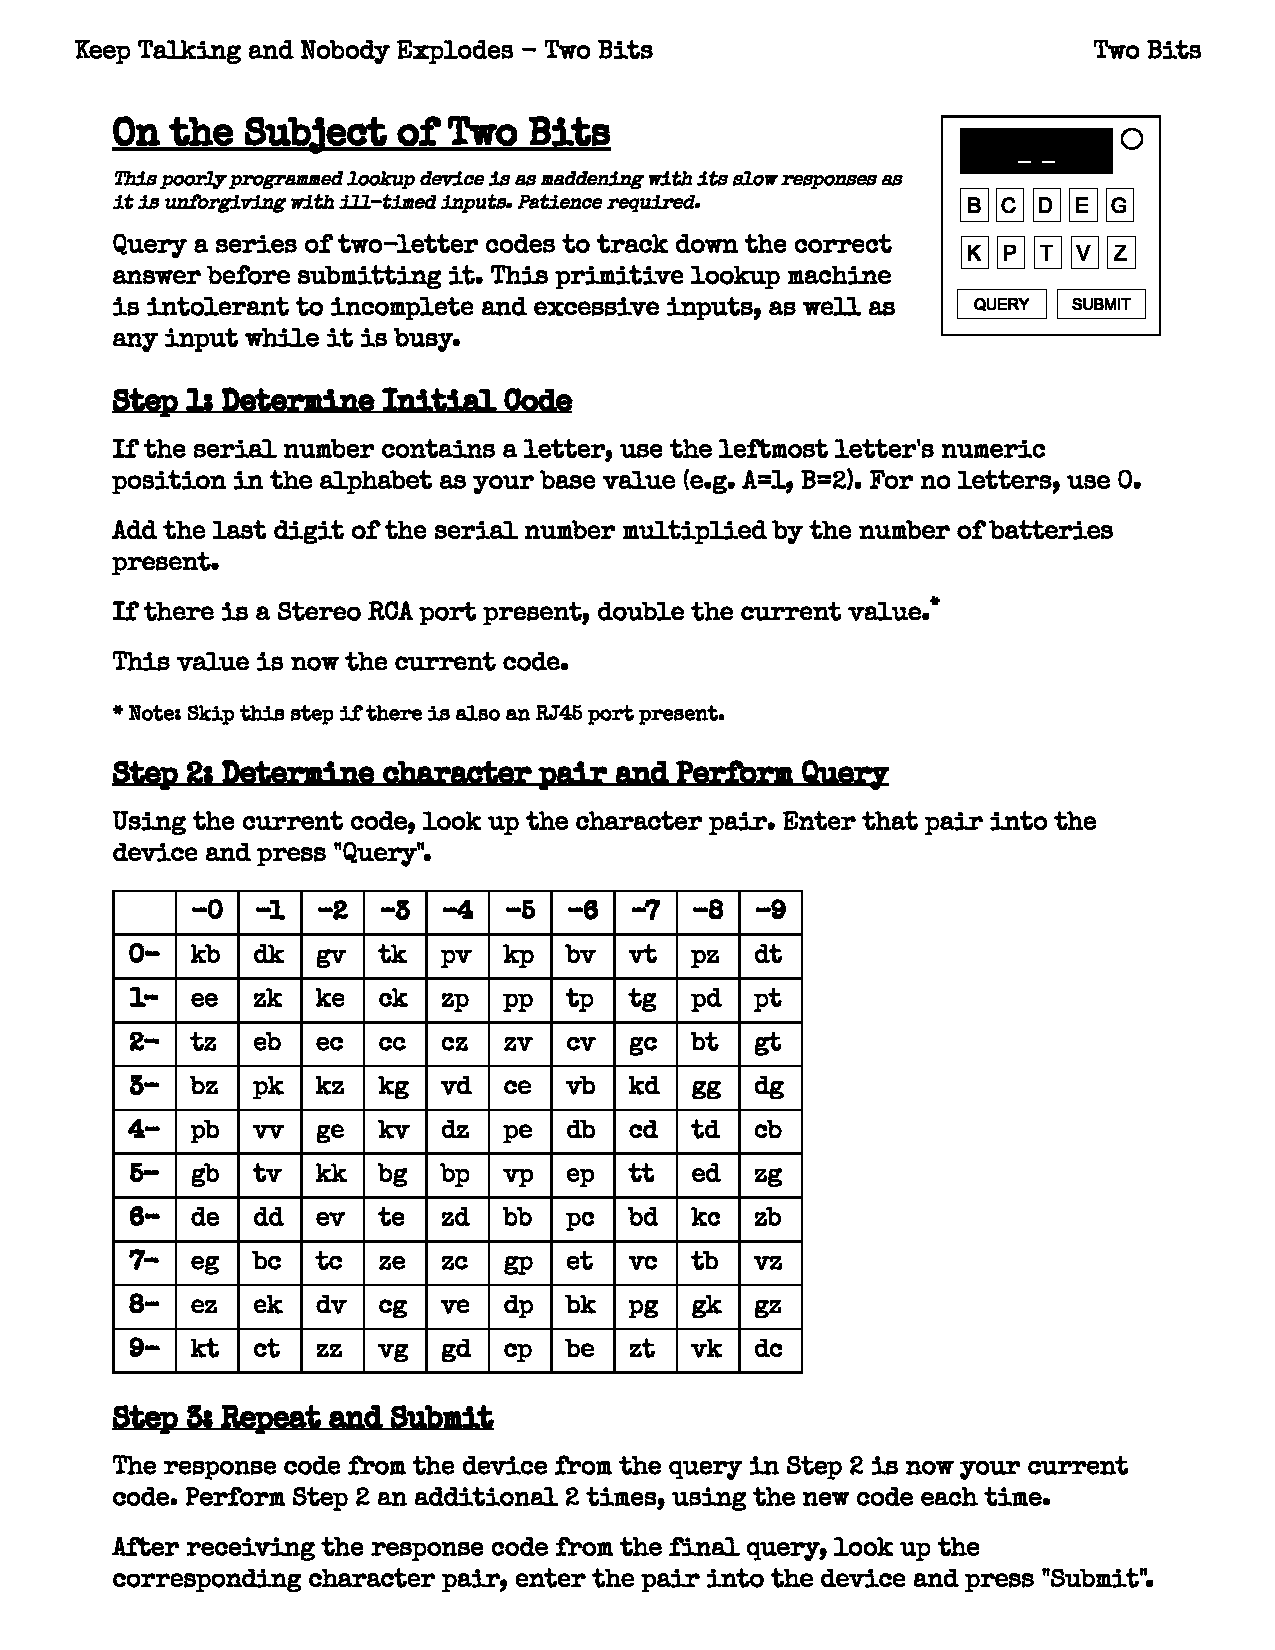
\includepdf[scale=0.9,pages=-,pagecommand={}]{pdf/6buttons/twoBits.pdf}

\newpage
\vspace*{-4cm}
\centerline{
\begin{overpic}[scale=1.0,unit=1mm,page=1]{pdf/text/SeaShells.pdf}
    \put(160,20){
\includegraphics{attention.png}}
\end{overpic}
}

\newpage
 
\includepdf[scale=0.9,pages=-,pagecommand={}]{pdf/text/EnglishTest.pdf}

\newpage
\invisiblesection{See Through}
\vspace*{-4cm}
\centerline{
\begin{overpic}[scale=0.9,unit=1mm,page=9]{pdf/sections.pdf}
\end{overpic}
}

\newpage
\thispagestyle{empty}
\mbox{}

\newpage
\vspace*{-4cm}
\centerline{
\begin{overpic}[scale=1.0,unit=1mm,page=16]{pdf/vanilla.pdf}
    \put(160,20){
\includegraphics{attention.png}}
\end{overpic}
}

\newpage
 
\includepdf[pages=12,pagecommand={}]{pdf/vanilla.pdf}

\newpage
 
\includepdf[pages=6-7,pagecommand={}]{pdf/advanced.pdf}

\newpage
 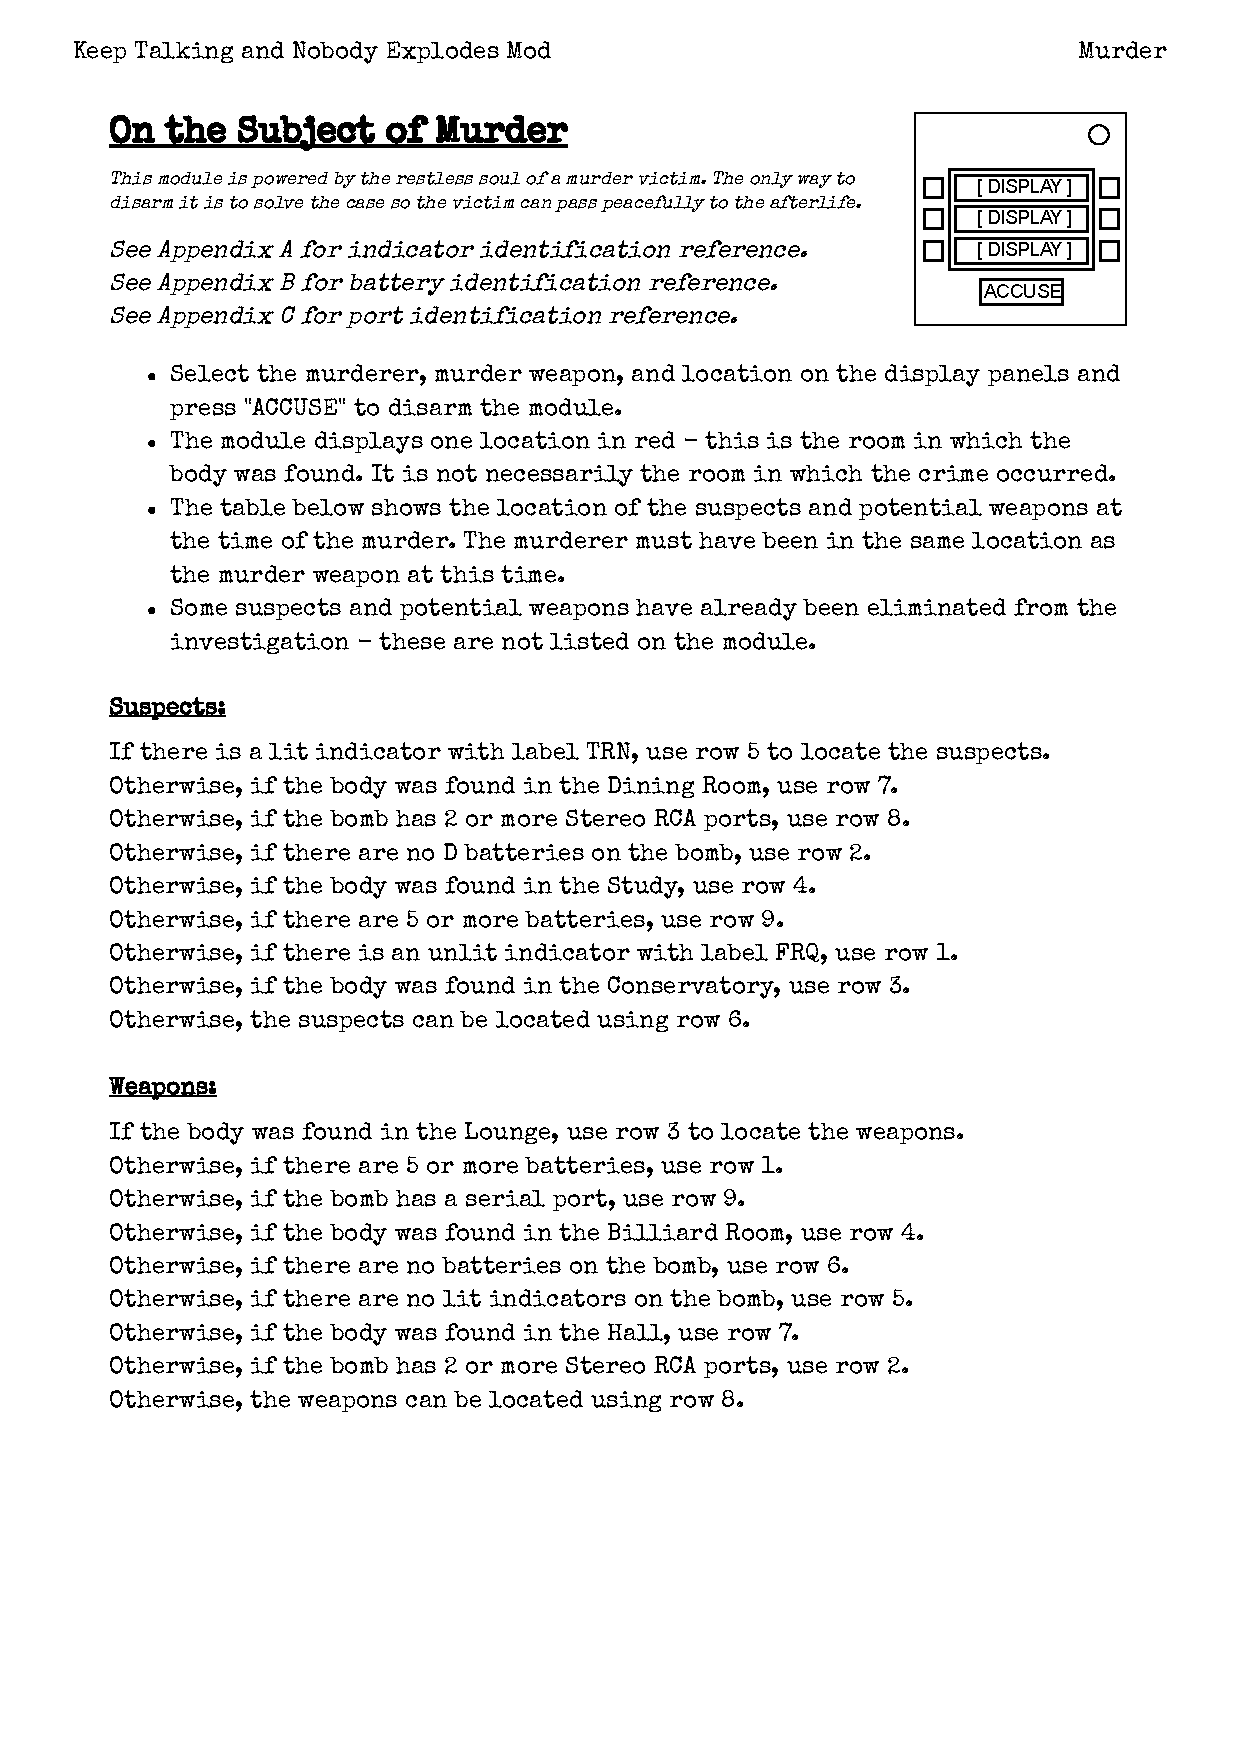
\includepdf[pages=-,pagecommand={}]{pdf/seethrough/Murder.pdf}

\newpage
 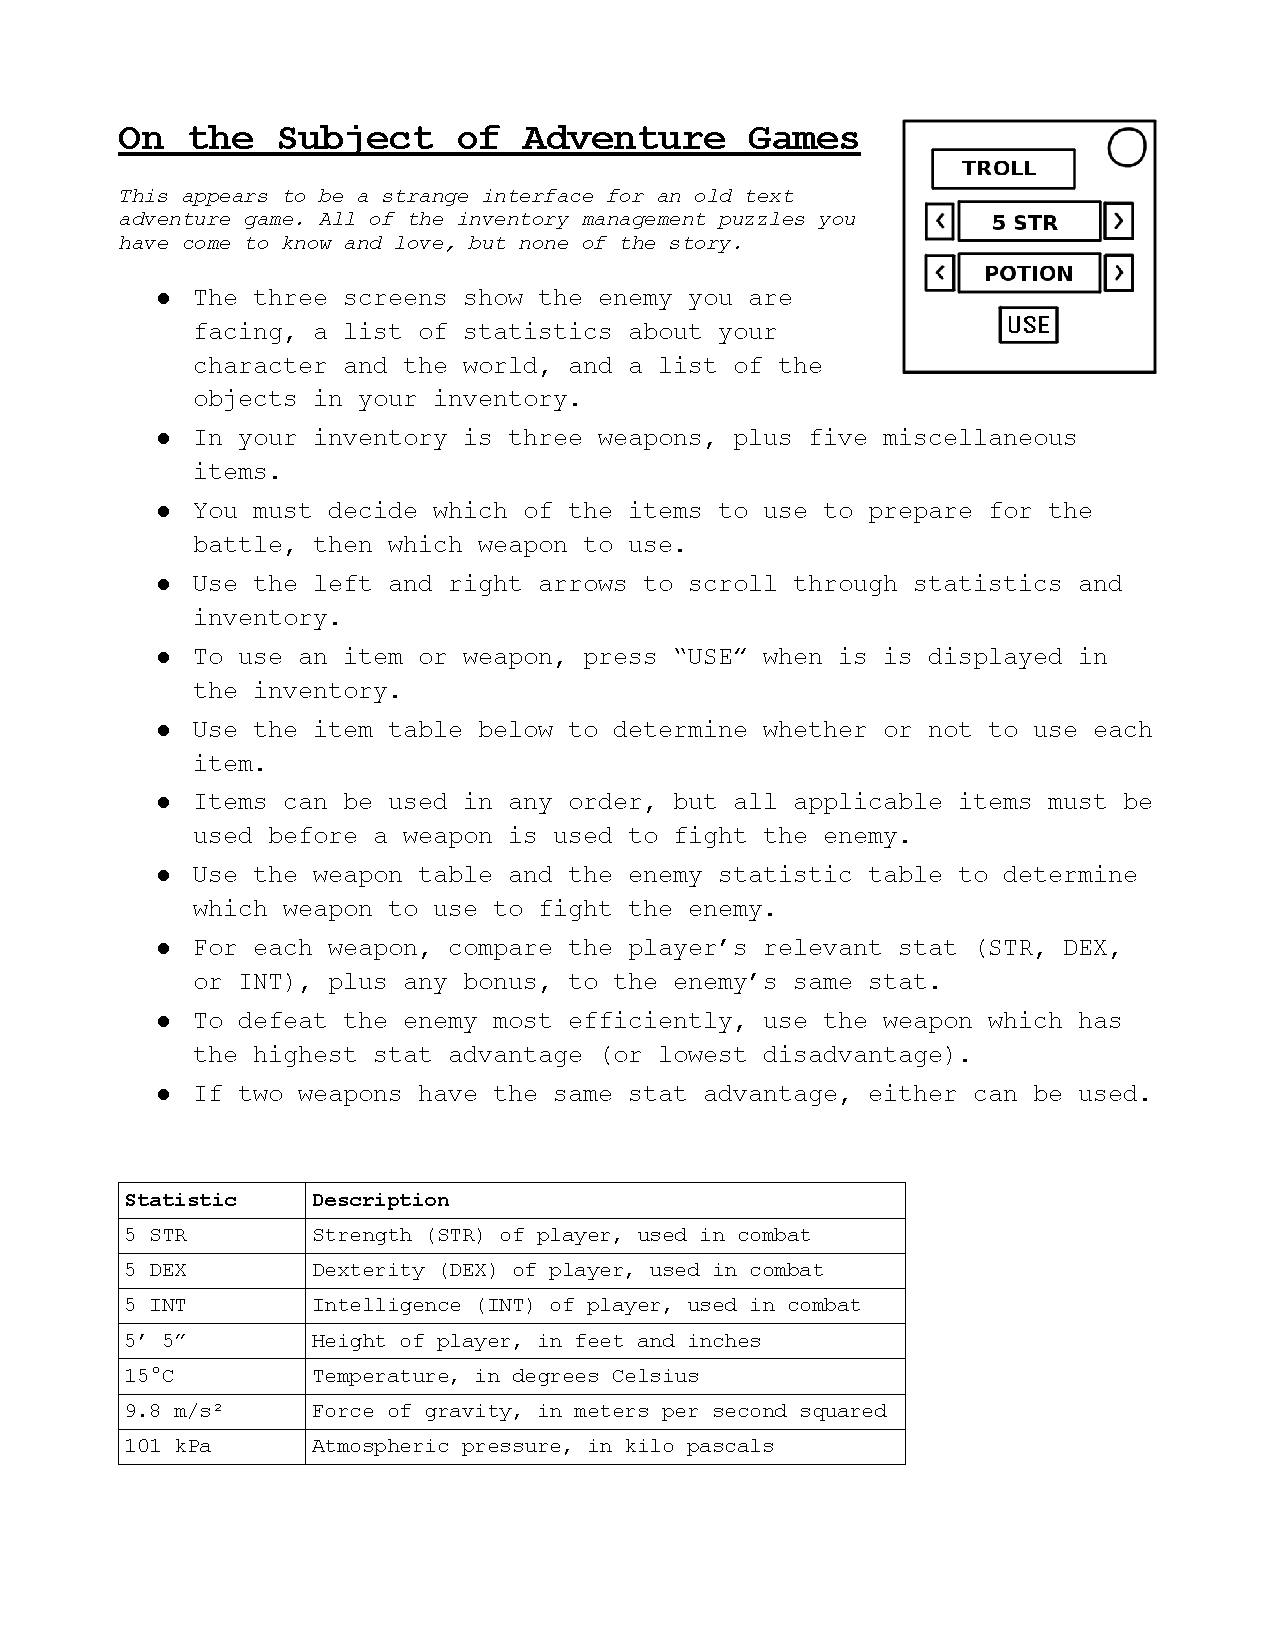
\includepdf[pages=-,pagecommand={}]{pdf/seethrough/AdventureGame.pdf}

\newpage
 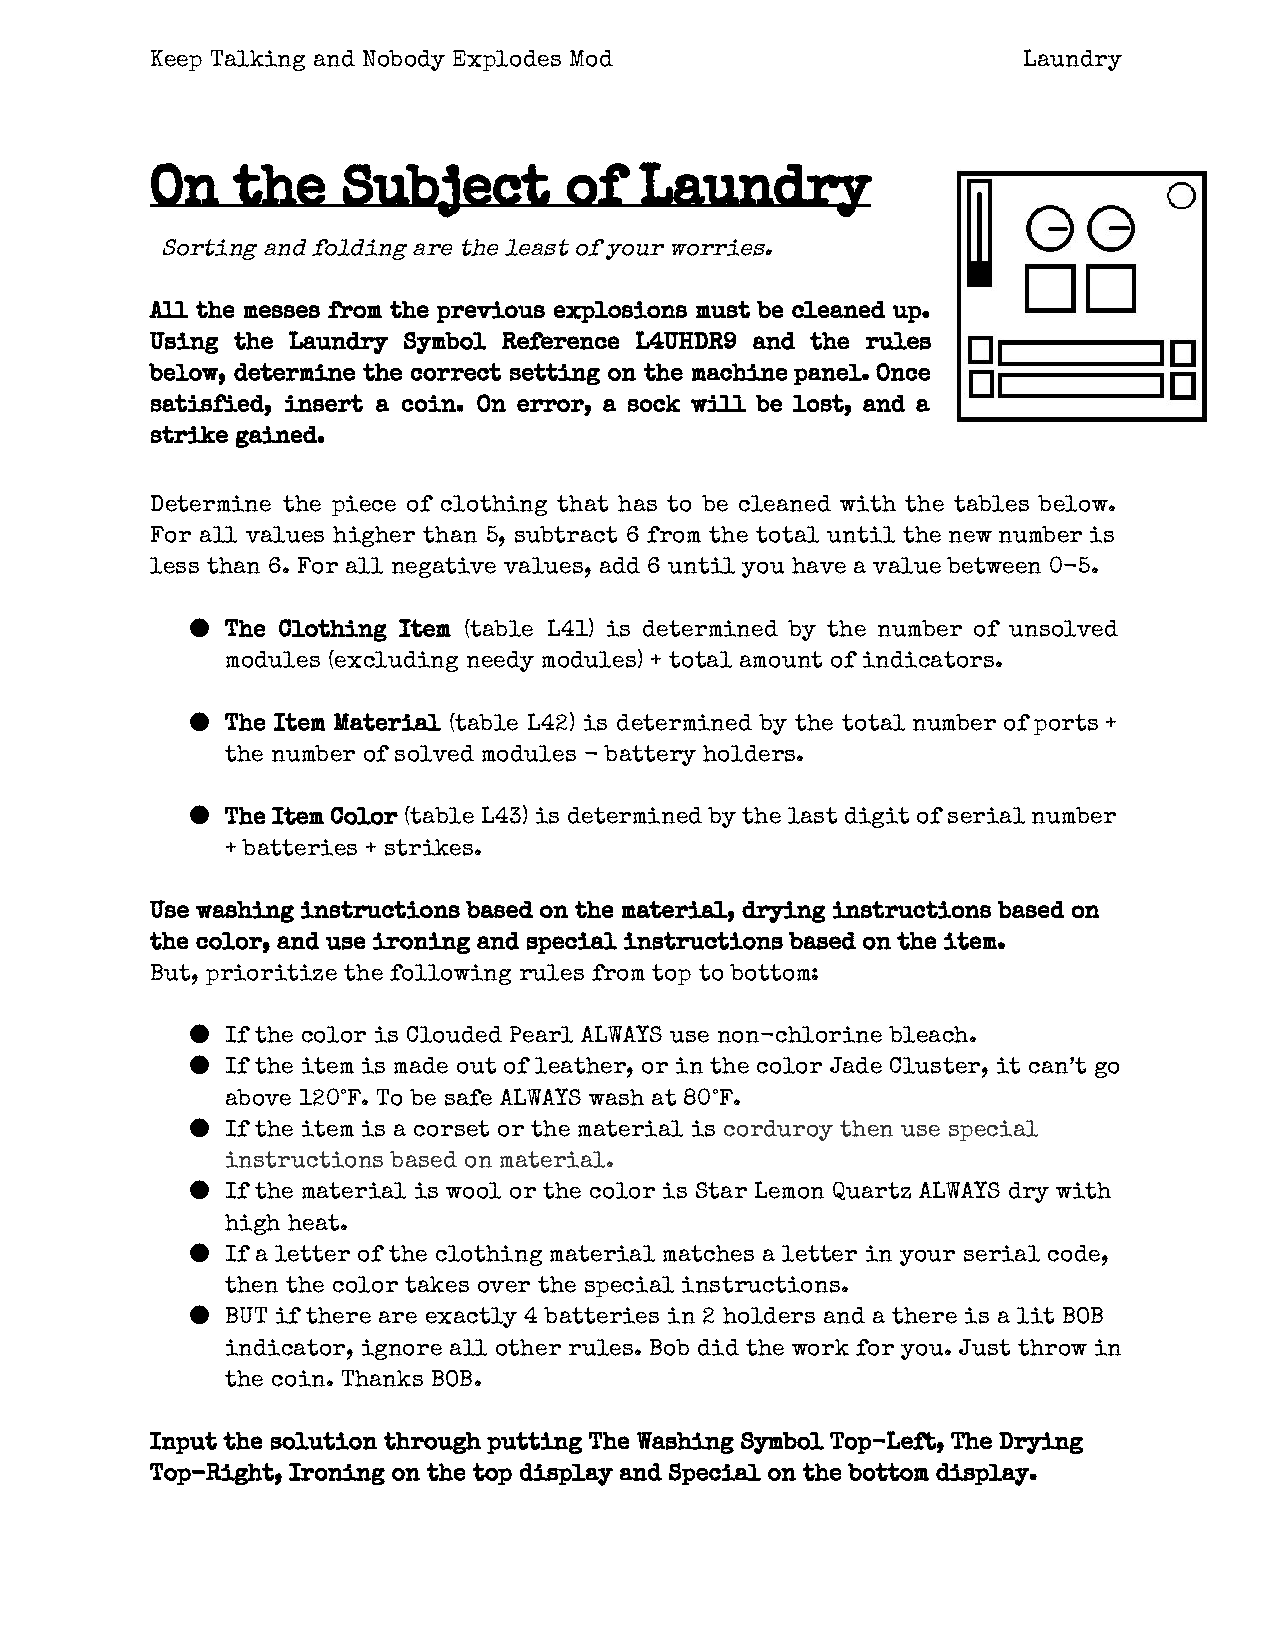
\includepdf[scale=1.0,pages=1-2,pagecommand={}]{pdf/seethrough/OnTheSubjectofLaundry.pdf}

\newpage
\vspace*{-4cm}
\centerline{
\begin{overpic}[scale=0.85,unit=1mm,page=3]{pdf/seethrough/OnTheSubjectofLaundry.pdf}
    \put(160,20){
\includegraphics{attention.png}}
\end{overpic}
}

\newpage
 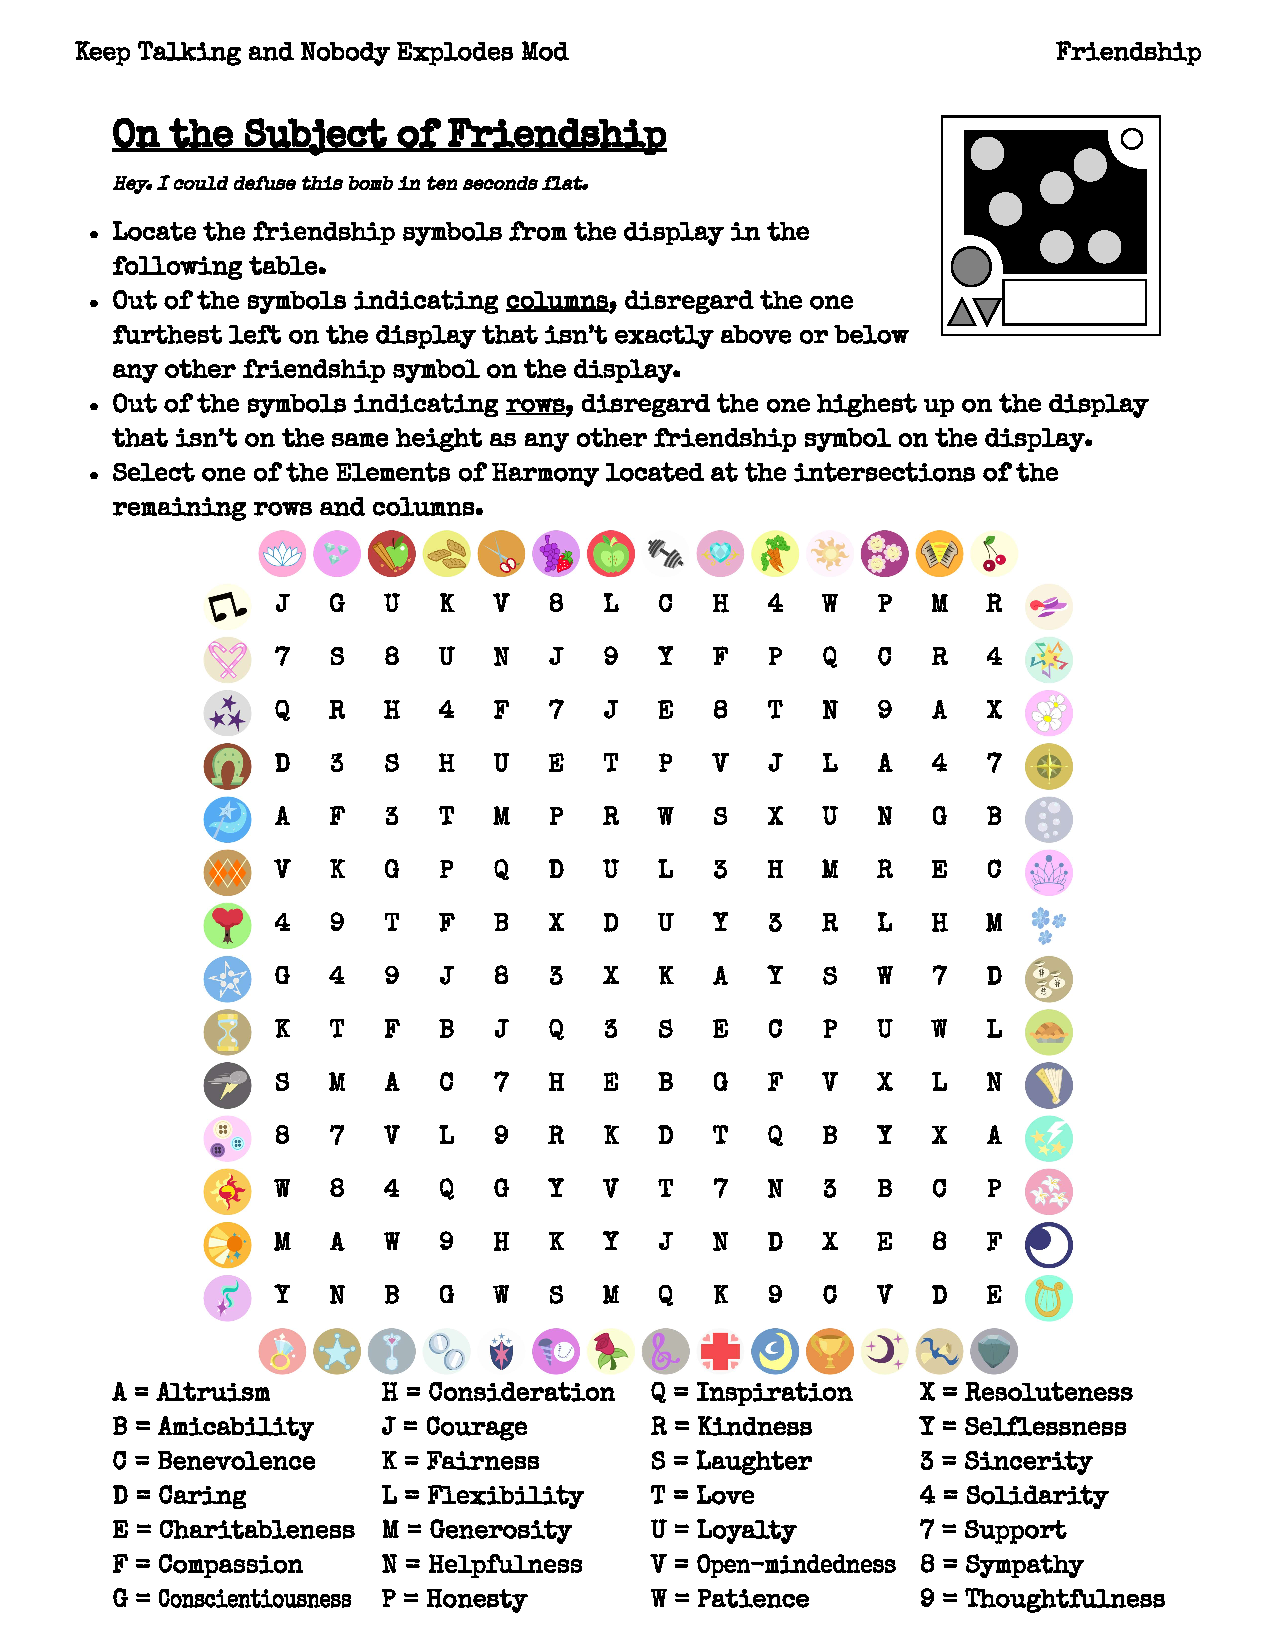
\includepdf[scale=0.9,pages=-,pagecommand={}]{pdf/seethrough/friendship.pdf}

\newpage
 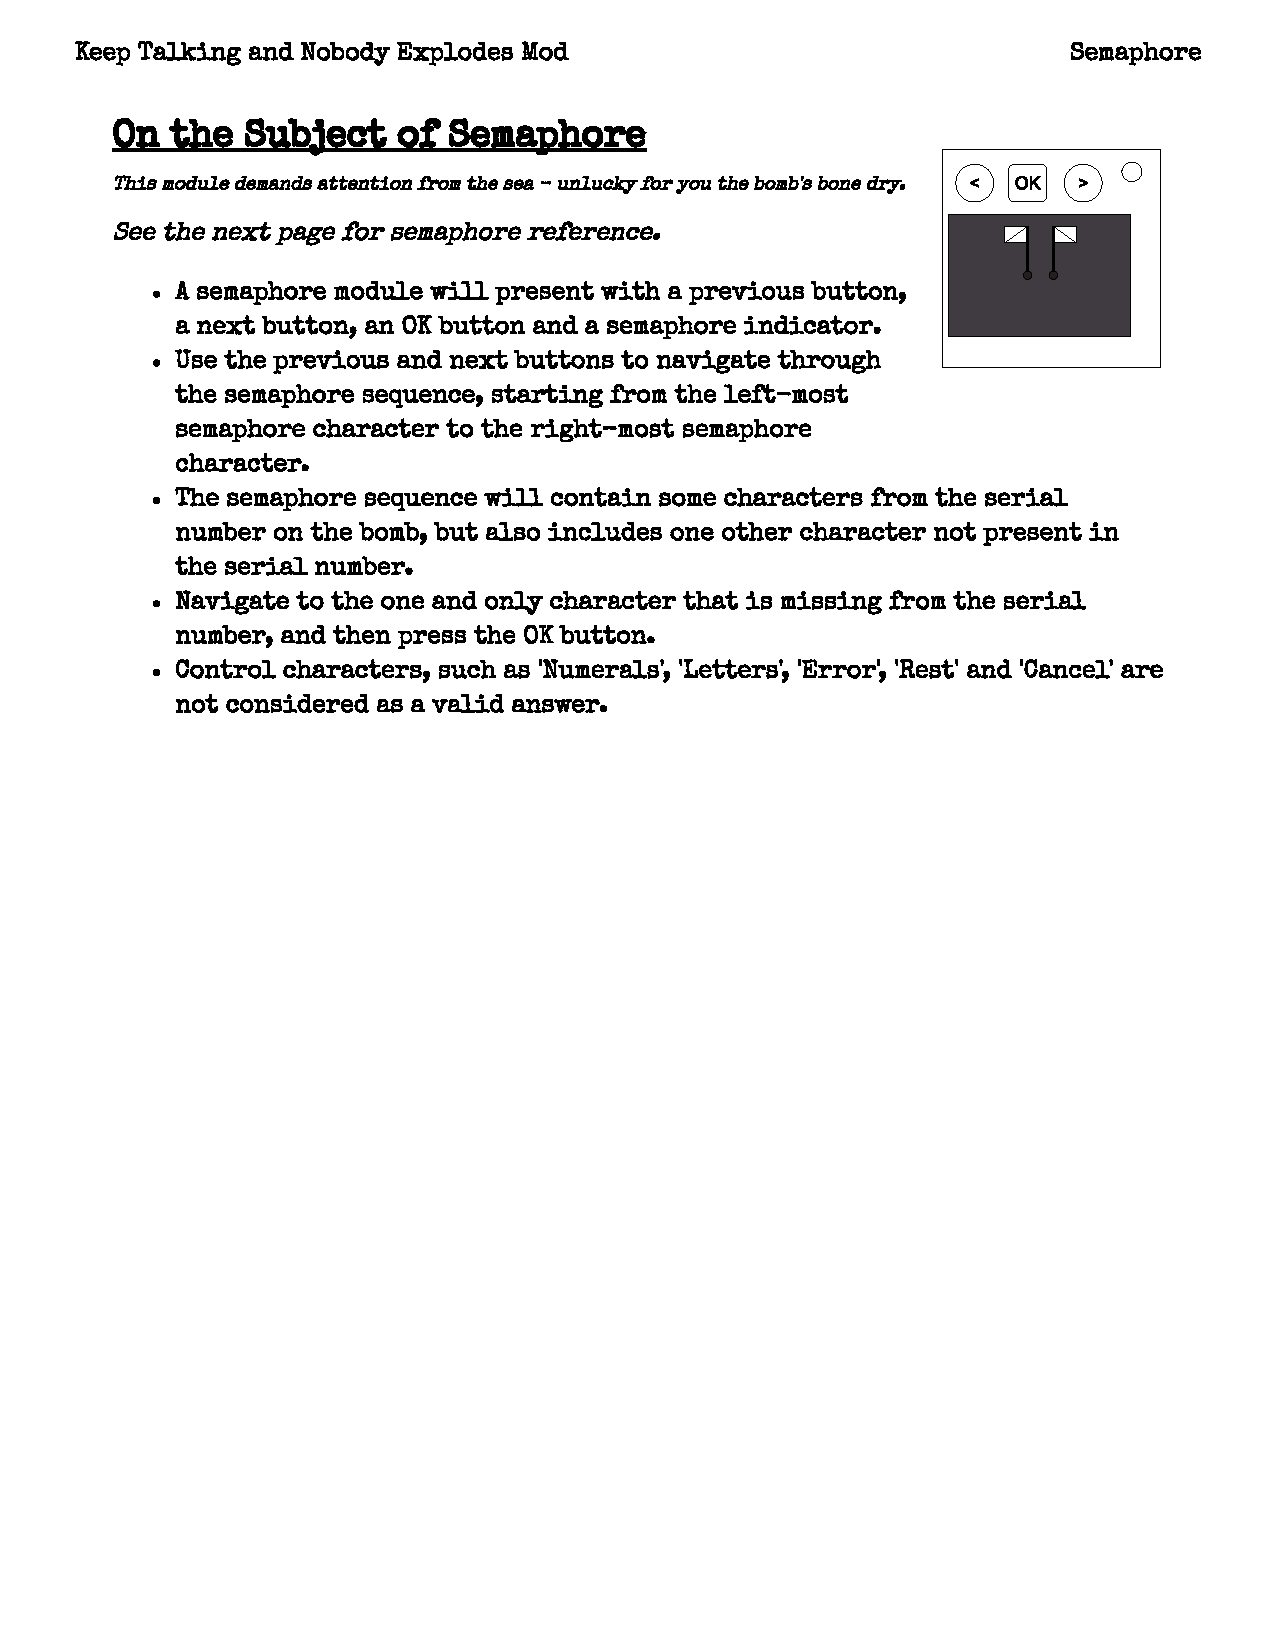
\includepdf[pages=-,pagecommand={}]{pdf/seethrough/semaphore.pdf}

\invisiblesection{Boolean}
 \includepdf[pages=10,pagecommand={}]{pdf/sections.pdf}

\newpage
\thispagestyle{empty}
\mbox{}

\newpage
 \includepdf[scale=0.9,pages=-,pagecommand={}]{pdf/boolean/colourflash.pdf}

\newpage
\vspace*{-4cm}
\centerline{
\begin{overpic}[scale=1.0,unit=1mm,page=1]{pdf/boolean/Logic.pdf}
    \put(180,30){\includegraphics{attention.png}}
\end{overpic}
}

\newpage
 \includepdf[pages=-,pagecommand={}]{pdf/boolean/SillySlots.pdf}

\newpage
 \includepdf[pages=-,pagecommand={}]{pdf/boolean/ConnectionCheckManual.pdf}

\newpage
 \includepdf[pages=-,pagecommand={}]{pdf/boolean/TheBulb.pdf}

\newpage
 \includepdf[pages=-,pagecommand={}]{pdf/boolean/switches.pdf}

\newpage
\thispagestyle{empty}
\mbox{}


\invisiblesection{Expert}
 \includepdf[pages=11,pagecommand={}]{pdf/sections.pdf}

\newpage
\thispagestyle{empty}
\mbox{}

\newpage
 \includepdf[scale=0.95,pages=-,pagecommand={}]{pdf/expert/NumberPad.pdf}

\newpage
 \includepdf[pages=-,pagecommand={}]{pdf/expert/3DMazeManual.pdf}

\newpage
\thispagestyle{empty}
\mbox{}

\newpage
\vspace*{-4cm}
\centerline{
\begin{overpic}[scale=1.0,unit=1mm,page=2]{pdf/advanced.pdf}
    \put(160,20){\includegraphics{attention.png}}
\end{overpic}
}

\newpage
 \includepdf[pages=3,pagecommand={}]{pdf/advanced.pdf}

\newpage
 \includepdf[pages=4-5,pagecommand={}]{pdf/advanced.pdf}

\newpage
 \includepdf[pages=-,pagecommand={}]{pdf/expert/CruelPianoKeys.pdf}

\newpage
\thispagestyle{empty}
\mbox{}

\invisiblesection{Other}
 \includepdf[pages=12,pagecommand={}]{pdf/sections.pdf}

\newpage
\thispagestyle{empty}
\mbox{}

\newpage
\vspace*{-4cm}
\centerline{
\begin{overpic}[scale=0.9,unit=1mm]{pdf/other/ShapeShift.pdf}
    \put(160,20){\includegraphics{attention.png}}
\end{overpic}
}

\newpage
 \includepdf[pages=-,pagecommand={}]{pdf/other/MouseInTheMaze.pdf}

\newpage
 \includepdf[pages=-,pagecommand={}]{pdf/other/PerspectivePegsManual.pdf}

\newpage
\includepdf[pages=-,pagecommand={}]{pdf/other/OrientationCube.pdf}

\newpage
\vspace*{-4cm}
\centerline{
\begin{overpic}[scale=0.7,unit=1mm]{pdf/other/Listening.pdf}
    \put(160,50){\includegraphics{attention.png}}
\end{overpic}
}

\newpage
 \includepdf[scale=0.9,pages=-]{pdf/other/combinationLock.pdf}

\newpage
 \includepdf[pages=1-2,pagecommand={}]{pdf/other/Astrology.pdf}

\newpage
\vspace*{-4cm}
\centerline{
\begin{overpic}[scale=1.0,page=3,unit=1mm]{pdf/other/Astrology.pdf}
    \put(160,50){\includegraphics{attention.png}}
\end{overpic}
}

\newpage
 \includepdf[pages=12]{pdf/vanilla.pdf}

\newpage
 \includepdf[pages=1-2,pagecommand={}]{pdf/other/SkewedSlots.pdf}


\invisiblesection{Needy}
\vspace*{-4cm}
\centerline{
\begin{overpic}[scale=0.9,unit=1mm,page=13]{pdf/sections.pdf}
\end{overpic}
}

\newpage
\thispagestyle{empty}
\mbox{}

\newpage
\vspace*{-4cm}
\centerline{
\begin{overpic}[scale=1.0,unit=1mm,page=18]{pdf/vanilla.pdf}
    \put(160,20){\includegraphics{attention.png}}
\end{overpic}
}

\newpage
 \includepdf[pages=19]{pdf/vanilla.pdf}

\newpage
\vspace*{-4cm}
\centerline{
\begin{overpic}[scale=1.0,unit=1mm,page=20]{pdf/vanilla.pdf}
    \put(160,20){\includegraphics{attention.png}}
\end{overpic}
}

\newpage
 \includepdf[pages=-]{pdf/needy/filibuster.pdf}

\newpage
\vspace*{-4cm}
\centerline{
\begin{overpic}[scale=1.0,unit=1mm]{pdf/needy/lightsOut.pdf}
    \put(160,20){\includegraphics{attention.png}}
\end{overpic}
}

\newpage
 \includepdf[pages=-]{pdf/needy/TetrisManual.pdf}

\newpage
\vspace*{-4cm}
\centerline{
\begin{overpic}[scale=1.0,unit=1mm]{pdf/needy/motionsense.pdf}
    \put(160,20){\includegraphics{attention.png}}
\end{overpic}
}

\newpage
 \includepdf[pages=-]{pdf/needy/MonsplodeWhoManual.pdf}

\newpage
\vspace*{-4cm}
\centerline{
\begin{overpic}[scale=1.0,unit=1mm,page=10]{pdf/advanced.pdf}
    \put(160,20){\includegraphics{attention.png}}
\end{overpic}
}

\newpage
 \includepdf[pages=11]{pdf/advanced.pdf}


\invisiblesection{Appendix}
\vspace*{-4cm}
\centerline{
\begin{overpic}[scale=0.9,unit=1mm,page=14]{pdf/sections.pdf}
\end{overpic}
}

\newpage
\thispagestyle{empty}
\mbox{}

\newpage
\vspace*{-4cm}
\centerline{
\begin{overpic}[scale=0.9,unit=1mm,page=21]{pdf/vanilla.pdf}
    \put(160,20){\includegraphics{attention.png}}
\end{overpic}
}

\newpage
 \includepdf[pages=22]{pdf/vanilla.pdf}


\newpage
\vspace*{-4cm}
\centerline{
\begin{overpic}[scale=1.0,unit=1mm,page=23]{pdf/vanilla.pdf}
    \put(160,20){\includegraphics{attention.png}}
\end{overpic}
}

\newpage
 \includepdf[pages=-]{pdf/appendix/TwoFactor.pdf}

\newpage
\vspace*{-4cm}
\centerline{
\begin{overpic}[scale=0.95,unit=1mm,page=1]{pdf/appendix/AppendixCD43.pdf}
\end{overpic}
}
 \includepdf[pages=-]{pdf/appendix/AppendixCD44.pdf}

\newpage
 \includepdf[pages=-,pagecommand={}]{pdf/appendix/EnglishTest.pdf}

\newpage
\vspace*{-4cm}
\centerline{
\begin{overpic}[scale=1.0,unit=1mm,page=12]{pdf/advanced.pdf}
    \put(160,20){\includegraphics{attention.png}}
\end{overpic}
}

\newpage
 \includepdf[pages=2]{pdf/other/GamePad.pdf}

\newpage
\vspace*{-4cm}
\centerline{
\begin{overpic}[scale=1.0,unit=1mm,page=3]{pdf/other/SkewedSlots.pdf}
\end{overpic}
}


\end{document}















